\PassOptionsToPackage{unicode,psdextra}{hyperref}
\documentclass[10pt,aspectratio=169]{beamer}

% <fonts>
\usefonttheme{professionalfonts}

\AtBeginSection[]{\frame{\sectionpage}}
\AtBeginSubsection[]{\frame{\subsectionpage}}
\setbeamertemplate{section page}
{
  \tableofcontents[
  currentsection,
  sectionstyle=show/shaded,
  subsectionstyle=hide,
  subsubsectionstyle=hide
  ]
}

\setbeamertemplate{subsection page}
{
  \tableofcontents[
  currentsection,
  sectionstyle=show/hide,
  subsectionstyle=show/shaded/hide,
  subsubsectionstyle=hide
  ]
}


\usepackage{fontspec}
\usepackage{fontawesome5}

\usepackage{mathtools}
\usepackage[mathrm=sym]{unicode-math}
\setmathfont{Fira Math}

\defaultfontfeatures{Scale = MatchUppercase}

\setmainfont{FiraSans}[
Path = /usr/local/texlive/2018/texmf-dist/fonts/opentype/public/fira/,
Extension = .otf ,
UprightFont = *-Regular,
BoldFont = *-Bold,
ItalicFont = *-Italic,
BoldItalicFont = *-BoldItalic]

\setsansfont{FiraSans}[
Path = /usr/local/texlive/2018/texmf-dist/fonts/opentype/public/fira/,
Extension = .otf ,
UprightFont = *-Regular,
BoldFont = *-Bold,
ItalicFont = *-Italic,
BoldItalicFont = *-BoldItalic]

\setmonofont{Fira Mono}
% </fonts>

\usepackage{esdiff}

\usepackage[french]{babel}

\useinnertheme{rectangles}
\useoutertheme{miniframes}

% https://tex.stackexchange.com/a/317833/8425
\makeatletter
\let\beamer@writeslidentry@miniframeson=\beamer@writeslidentry%
\def\beamer@writeslidentry@miniframesoff{%
  \expandafter\beamer@ifempty\expandafter{\beamer@framestartpage}{}% does not happen normally
  {%else
    % removed \addtocontents commands
    \clearpage\beamer@notesactions%
  }
}
\newcommand*{\miniframeson}{\let\beamer@writeslidentry=\beamer@writeslidentry@miniframeson}
\newcommand*{\miniframesoff}{\let\beamer@writeslidentry=\beamer@writeslidentry@miniframesoff}
\makeatother

% <colors>
\usepackage{xcolor-material}

\usecolortheme{whale}

\mode<presentation>
\setbeamercolor{alerted text}{fg = GoogleRed}
\setbeamercolor{example text}{fg = GoogleGreen}
\mode<all>


% https://tex.stackexchange.com/a/66475/8425
% Create Color definition From Template (both background and foreground colors): 
% #1 template name, 
% #2 foreground color name
% #3 background color name
\newcommand{\ccft}[3]{%
  \usebeamercolor{#1}
  \definecolor{#2}{named}{fg}
  \definecolor{#3}{named}{bg}
}

% Blocks color definition (background and foreground)
\ccft{block title}{block title fg}{block title bg}
\ccft{block body}{block body fg}{block body bg}
\ccft{block title alerted}{block title alerted fg}{block title alerted bg}
\ccft{block body alerted}{block body alerted fg}{block body alerted bg}
\ccft{block title example}{block title example fg}{block title example bg}
\ccft{block body example}{block body example fg}{block body example bg}
\ccft{primary}{primary fg}{primary bg}

\usepackage{pgffor, etextools}

\foreach \BeamerColor in {%
  structure, palette primary, palette secondary, palette tertiary, palette quaternary, palette sidebar primary, palette sidebar secondary, palette sidebar tertiary, palette sidebar quaternary, normal text, example text, titlelike, separation line}{%
  \ifbeamercolorempty[fg]{\expanded{\BeamerColor}}{}{%
    \usebeamercolor{\expanded{\BeamerColor}}\xglobal\definecolor{\expanded{\BeamerColor} fg}{named}{fg}
    \xappto\Rules{\noexpand\draw[ultra thick, \BeamerColor\space fg] (O) -- node[above, black, font = \noexpand\tiny]{\BeamerColor\space fg} ++(5,0) ++(-5, -.4) coordinate (O);}%
  }
  \ifbeamercolorempty[bg]{\expanded{\BeamerColor}}{}{%
    \usebeamercolor{\expanded{\BeamerColor}}\xglobal\definecolor{\expanded{\BeamerColor} bg}{named}{bg}
    \xappto\Rules{\noexpand\draw[ultra thick, \BeamerColor\space bg] (O) -- node[above, black, font = \noexpand\tiny]{\BeamerColor\space bg} ++(5,0) ++(-5, -.4) coordinate (O);}%
  }
}



% https://github.com/edasubert/beamerMaterialDesign
\definecolor{shadow}{HTML}{000000}
\definecolor{BGgrey01}{HTML}{E0E0E0}
\definecolor{BGgrey02}{HTML}{F5F5F5}
\definecolor{BGgrey03}{HTML}{FAFAFA}
\definecolor{BGgrey04}{HTML}{FFFFFF}

% </colors>

% <boxes>
\usepackage[most]{tcolorbox}

\newtcolorbox{Card}{%
  colback = BGgrey04,
  % colbacktitle = primary,
  % coltitle = textPrimary,
  % coltext = text,
  enhanced,
  sharpish corners = all,
  fuzzy shadow = {0mm}{0.9mm}{0.6mm}{0.2mm}{shadow!20!BGgrey03}, % top
  fuzzy shadow = {0mm}{-0.6mm}{-0.1mm}{0.2mm}{shadow!40!BGgrey03}, % bottomSmall
  fuzzy shadow = {0mm}{-0.2mm}{-0.2mm}{0.2mm}{shadow!20!BGgrey03}, % bottomBig
  left = 6mm, right = 6mm, top = 6mm, bottom = 6mm, middle = 4mm,
  notitle,
  boxrule = 0mm,
}

\newtcolorbox{Attention}{%
  colback = BGgrey04,
  % colbacktitle = primary,
  % coltitle = textPrimary,
  % coltext = text,
  enhanced,
  sharpish corners = all,
  fuzzy shadow = {0mm}{0.9mm}{0.6mm}{0.2mm}{shadow!20!BGgrey03}, % top
  fuzzy shadow = {0mm}{-0.6mm}{-0.1mm}{0.2mm}{shadow!40!BGgrey03}, % bottomSmall
  fuzzy shadow = {0mm}{-0.2mm}{-0.2mm}{0.2mm}{shadow!20!BGgrey03}, % bottomBig
  left = 6mm, right = 6mm, top = 6mm, bottom = 6mm, middle = 4mm,
  notitle,
  boxrule = 0mm,
  leftrule = 12mm,
  colframe = GoogleRed,
  overlay = {%
    \node[anchor = north, font = \huge] at ([xshift = 6mm]frame.north west) {\color{white}\faExclamationCircle};},
}

\newtcolorbox{BonASavoir}{%
  colback = BGgrey04,
  % colbacktitle = primary,
  % coltitle = textPrimary,
  % coltext = text,
  enhanced,
  sharpish corners = all,
  fuzzy shadow = {0mm}{0.9mm}{0.6mm}{0.2mm}{shadow!20!BGgrey03}, % top
  fuzzy shadow = {0mm}{-0.6mm}{-0.1mm}{0.2mm}{shadow!40!BGgrey03}, % bottomSmall
  fuzzy shadow = {0mm}{-0.2mm}{-0.2mm}{0.2mm}{shadow!20!BGgrey03}, % bottomBig
  left = 6mm, right = 6mm, top = 6mm, bottom = 6mm, middle = 4mm,
  notitle,
  boxrule = 0mm,
  leftrule = 12mm,
  colframe = MaterialAmber,
  overlay = {%
    \node[anchor = north, font = \huge] at ([xshift = 6mm]frame.north west) {\color{white}\faInfoCircle};},
}

\newtcolorbox{Conseil}{%
  colback = BGgrey04,
  % colbacktitle = primary,
  % coltitle = textPrimary,
  % coltext = text,
  enhanced,
  sharpish corners = all,
  fuzzy shadow = {0mm}{0.9mm}{0.6mm}{0.2mm}{shadow!20!BGgrey03}, % top
  fuzzy shadow = {0mm}{-0.6mm}{-0.1mm}{0.2mm}{shadow!40!BGgrey03}, % bottomSmall
  fuzzy shadow = {0mm}{-0.2mm}{-0.2mm}{0.2mm}{shadow!20!BGgrey03}, % bottomBig
  left = 6mm, right = 6mm, top = 6mm, bottom = 6mm, middle = 4mm,
  notitle,
  boxrule = 0mm,
  leftrule = 12mm,
  colframe = example text fg,
  overlay = {%
    \node[anchor = north, font = \Large] at ([xshift = 6mm]frame.north west) {\color{white}\faThumbsUp[solid]};},
}

\undef\Definition
\undef\endDefinition

\newtcolorbox{Definition}{%
  colback = BGgrey04,
  % colbacktitle = primary,
  % coltitle = textPrimary,
  % coltext = text,
  enhanced,
  sharpish corners = all,
  fuzzy shadow = {0mm}{0.9mm}{0.6mm}{0.2mm}{shadow!20!BGgrey03}, % top
  fuzzy shadow = {0mm}{-0.6mm}{-0.1mm}{0.2mm}{shadow!40!BGgrey03}, % bottomSmall
  fuzzy shadow = {0mm}{-0.2mm}{-0.2mm}{0.2mm}{shadow!20!BGgrey03}, % bottomBig
  left = 6mm, right = 6mm, top = 6mm, bottom = 6mm, middle = 4mm,
  notitle,
  boxrule = 0mm,
  leftrule = 12mm,
  colframe = MaterialDeepOrange,
  overlay = {%
    \node[anchor = north, font = \Large] at ([xshift = 6mm]frame.north west) {\color{white}\faBookOpen[solid]};},
}


\usepackage{fancyvrb}
\usepackage{minted}
\tcbuselibrary{minted}

\renewcommand{\theFancyVerbLine}{%
  \sffamily
  \small
  {\color{white}\arabic{FancyVerbLine}}}

\newtcbinputlisting{\includepythonfile}[2][Script Python]{%
  enhanced,
  sharpish corners = all,
  fuzzy shadow = {0mm}{0.9mm}{0.6mm}{0.2mm}{shadow!20!BGgrey03}, % top
  fuzzy shadow = {0mm}{-0.6mm}{-0.1mm}{0.2mm}{shadow!40!BGgrey03}, % bottomSmall
  fuzzy shadow = {0mm}{-0.2mm}{-0.2mm}{0.2mm}{shadow!20!BGgrey03}, % bottomBig
  left = 6mm, right = 6mm, top = 6mm, bottom = 6mm, middle = 4mm,
  colbacktitle = normal text bg, 
  coltitle = GoogleRed, 
  colback = palette sidebar primary fg,
  fonttitle = \scriptsize\bfseries,
  title = {\faPython~#1 (\texttt{#2})},
  overlay = {%
    \begin{tcbclipinterior}
      \fill[palette sidebar tertiary fg] (frame.south west) rectangle ([xshift=5mm]frame.north west);
    \end{tcbclipinterior}
  },
  listing engine = minted,
  minted language = python,
  minted style = colorful,
  minted options = {%
    fontsize = \small,
    linenos,
    numbersep = 3mm},
  listing file = python/#2,
  boxrule = .5pt,
  listing only,
}

% </boxes>

\title{Une introduction à Python}

\institute[]{Lycée Jacques Decour -- Paris}

\author[C. Jorssen]{%
  Christophe Jorssen\\
  \footnotesize\href{mailto:christophe.jorssen@gmail.com}{christophe.jorssen@gmail.com} \\
  \footnotesize\url{https://github.com/cjorssen/presentation-python-JD}}

\date{Jeudi 4 avril 2019}

\begin{document}

\begin{frame}
  \titlepage
\end{frame}

\begin{frame}
  \includepythonfile{hello.py}
\end{frame}

\begin{frame}{Plan}
  \tableofcontents[hideallsubsections]
\end{frame}

\section{Un peu de « vécu »}

\subsection{Oscillateur quasi sinusoïdal}

\begin{frame}
  \begin{columns}
    \begin{column}{.5\linewidth}
    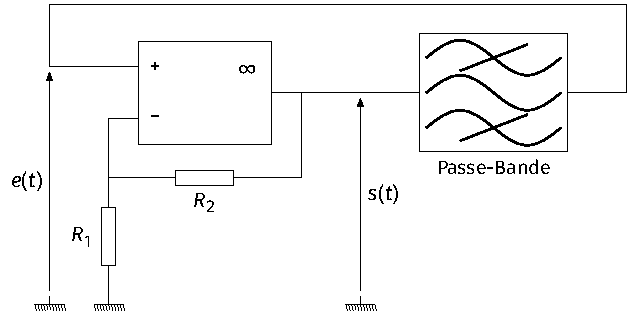
\includegraphics[width = \linewidth]{schema-oscillateur-QS-boucle}
  \end{column}
  \begin{column}{.5\linewidth}
    Système non linéaire :
    \begin{itemize}
    \item si $|G e| < V_{\mathrm{sat}}$, alors $$\diff[2]{s}{t} + (1 - G H_0) \frac{\omega_0}{Q} \diff{s}{t} + \omega_0^2 s = 0 ;$$
    \item si $|G e| \geqslant V_{\mathrm{sat}}$, alors $$\diff[2]{s}{t} + \frac{\omega_0}{Q} \diff{s}{t} + \omega_0^2 s = 0.$$
    \end{itemize}

  \end{column}
\end{columns}
\end{frame}

\begin{frame}
  \centering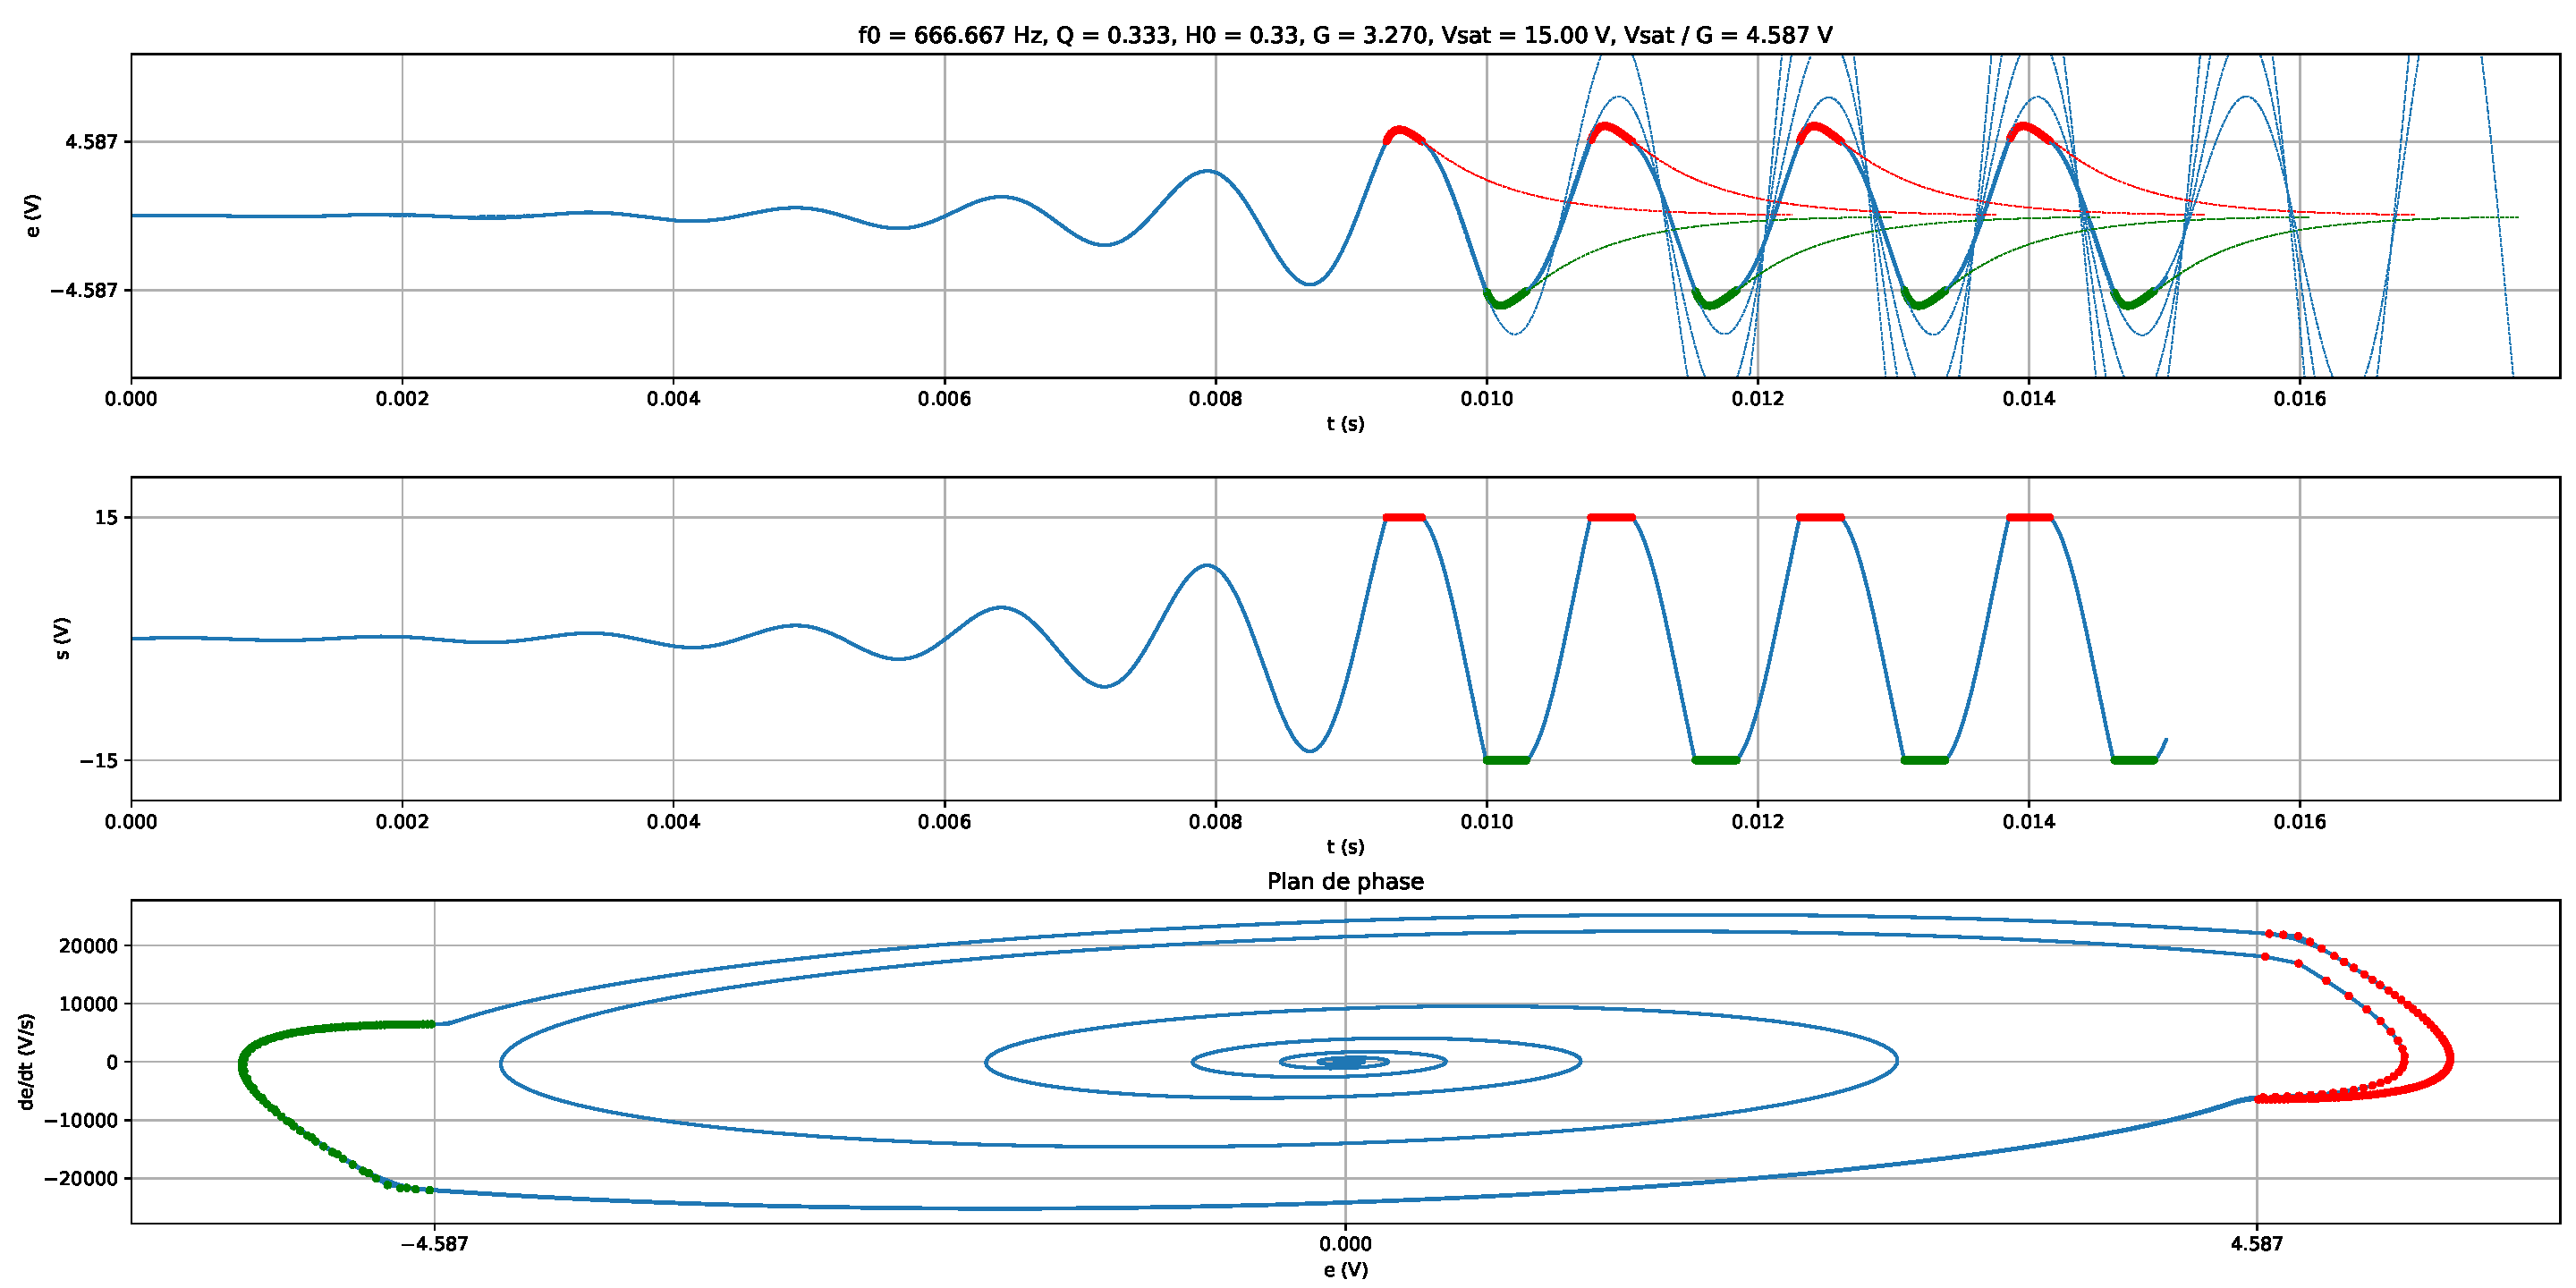
\includegraphics[height = .9\textheight]{plot-oscillateur-QS-python}
\end{frame}

\subsection{Trajectoire d'un projectile}

\subsection{Propagation d'un paquet d'onde}

\subsection{Analyse spectrale du son d'une flûte, mode propres d'une corde pincée}

\subsection{Propagation d'une onde le long d'une « échelle de perroquet »}


\section{Installation et mise à jour de l'écosystème Python}

\subsection{Nécessité d'une distribution}

\begin{frame}
  Ne jamais installer « à la main » les différents constituants de l'écosystème Python.
  \begin{Conseil}
    Installer une \alert{distribution} proposant, entre autres :
    \begin{itemize}
    \item un \alert{IDE} (\emph{integrated development environment}) ;
    \item un \alert{gestionnaire de paquets}.
    \end{itemize}
  \end{Conseil}
\end{frame}

\begin{frame}{Les distributions}
  \begin{description}
  \item[Pyzo] \url{https://pyzo.org/}
  \item[Anaconda] \alert{\faHandPointRight[regular]}\url{https://www.anaconda.com/distribution/}\alert{\faHandPointLeft[regular]}
  \end{description}
\end{frame}

\begin{frame}{La distribution Anaconda}
  \begin{itemize}
  \item Installe les outils nécessaires à une \alert{utilisation scientifique} (au sens large) de Python.
  \item Installe un IDE dédié à Python : \alert{spyder}.
  \item Installe un gestionnaire de paquet avancé : \alert{conda}.
  \item Installe une \alert{interface graphique} permettant une utilisation « à la souris » de la distribution et de ses outils.
  \end{itemize}
\end{frame}

\subsection{Installation d'Anaconda}

\begin{frame}
  \begin{Attention}
    Lors de l'installation de Python, il faut :
    \begin{itemize}
    \item faire attention à ce que le Python nouvellement installé \alert{ne perturbe pas} un Python déjà installé ;
    \item faire en sorte que le Python que l'on utilise soit \alert{trouvé} ;
    \item faire en sorte que le Python que l'on utilise soit \alert{le bon}.
    \end{itemize}
  \end{Attention}
\end{frame}

\begin{frame}{Installation d'Anaconda (MS-Windows)}
  \begin{center}
    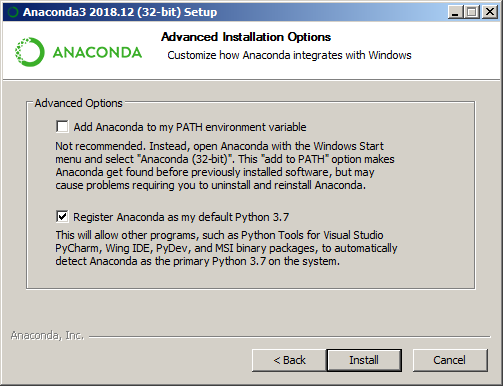
\includegraphics[height = .8\textheight]{installation-anaconda-win-interaction-systeme}
  \end{center}
\end{frame}

\begin{frame}{Installation d'Anaconda (MS-Windows)}
  \begin{center}
    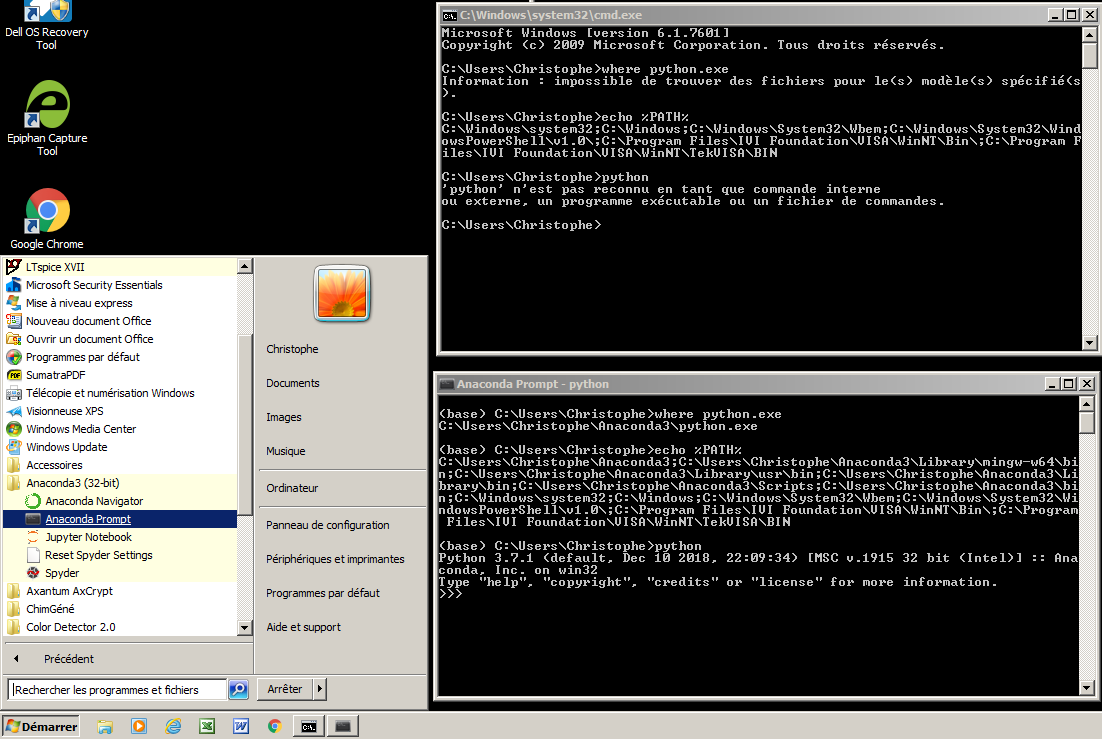
\includegraphics[height = .8\textheight]{anaconda-prompt-vs-cmd-windows.png}
  \end{center}
\end{frame}

\begin{frame}{Installation d'Anaconda (MacOS)}
  \begin{center}
    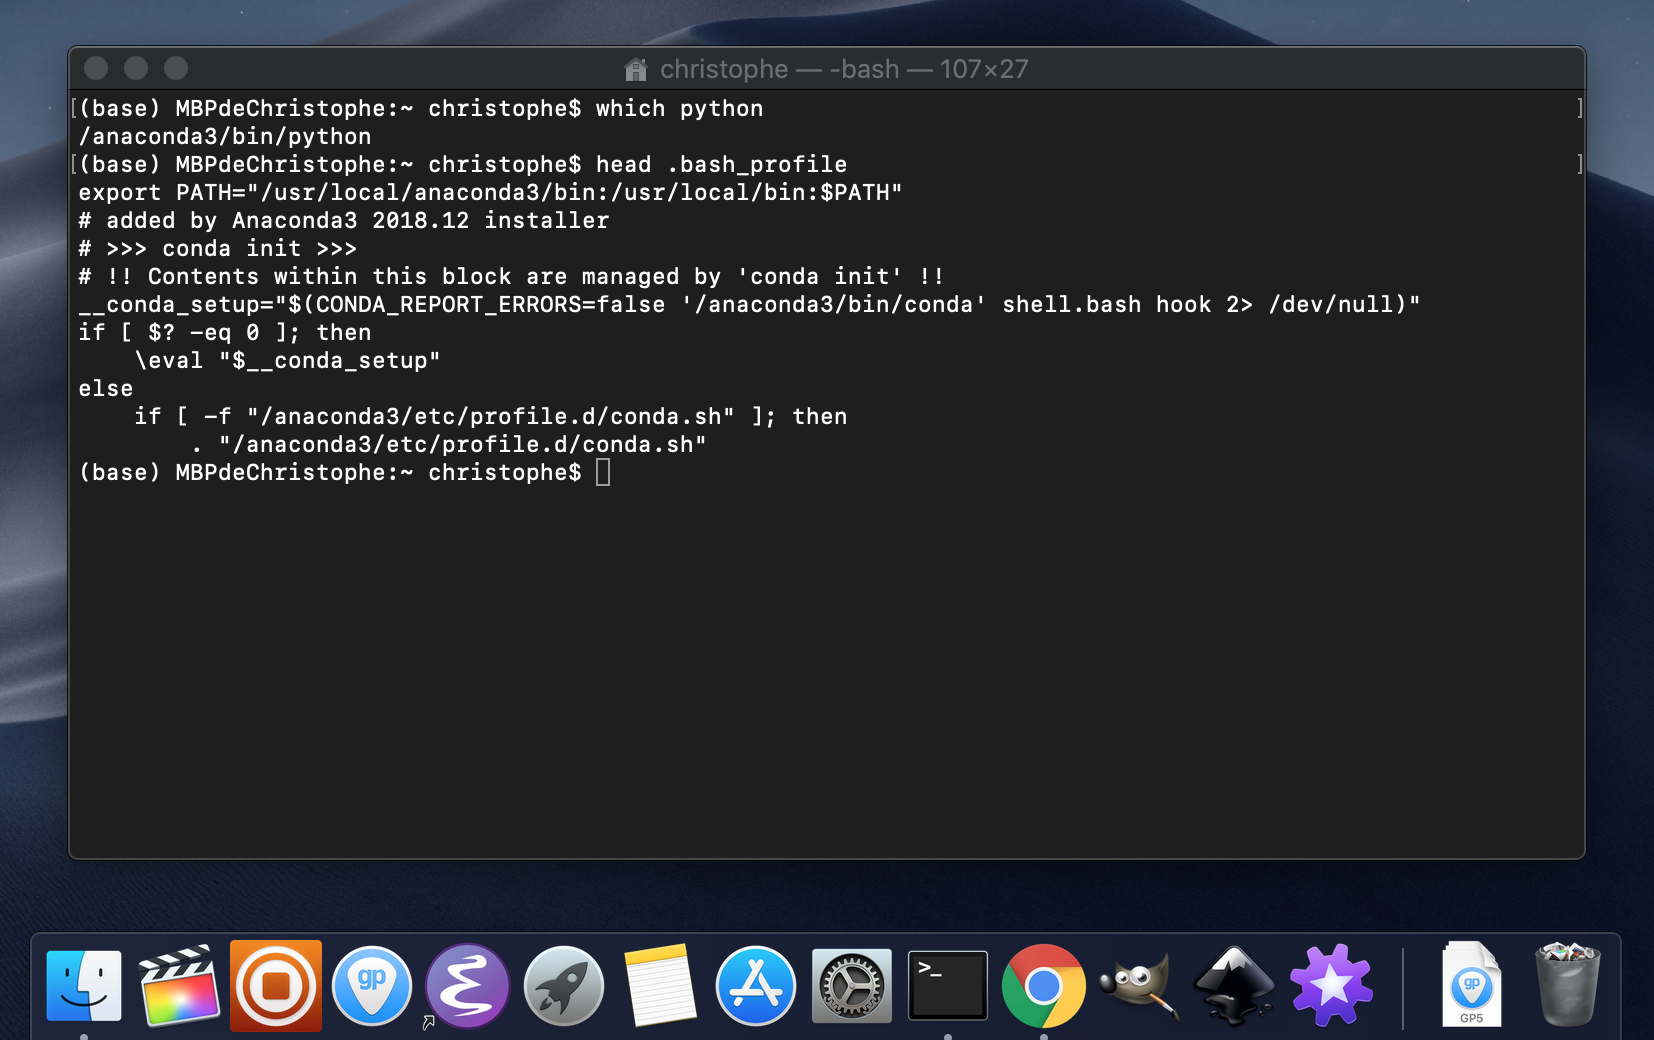
\includegraphics[height = .8\textheight]{prompt-terminal-macos}
  \end{center}
\end{frame}

\subsection{Mise à jour et installation de paquets complémentaires}

\begin{frame}{À l'aide de l'interface graphique : mise à jour}
  \begin{center}
    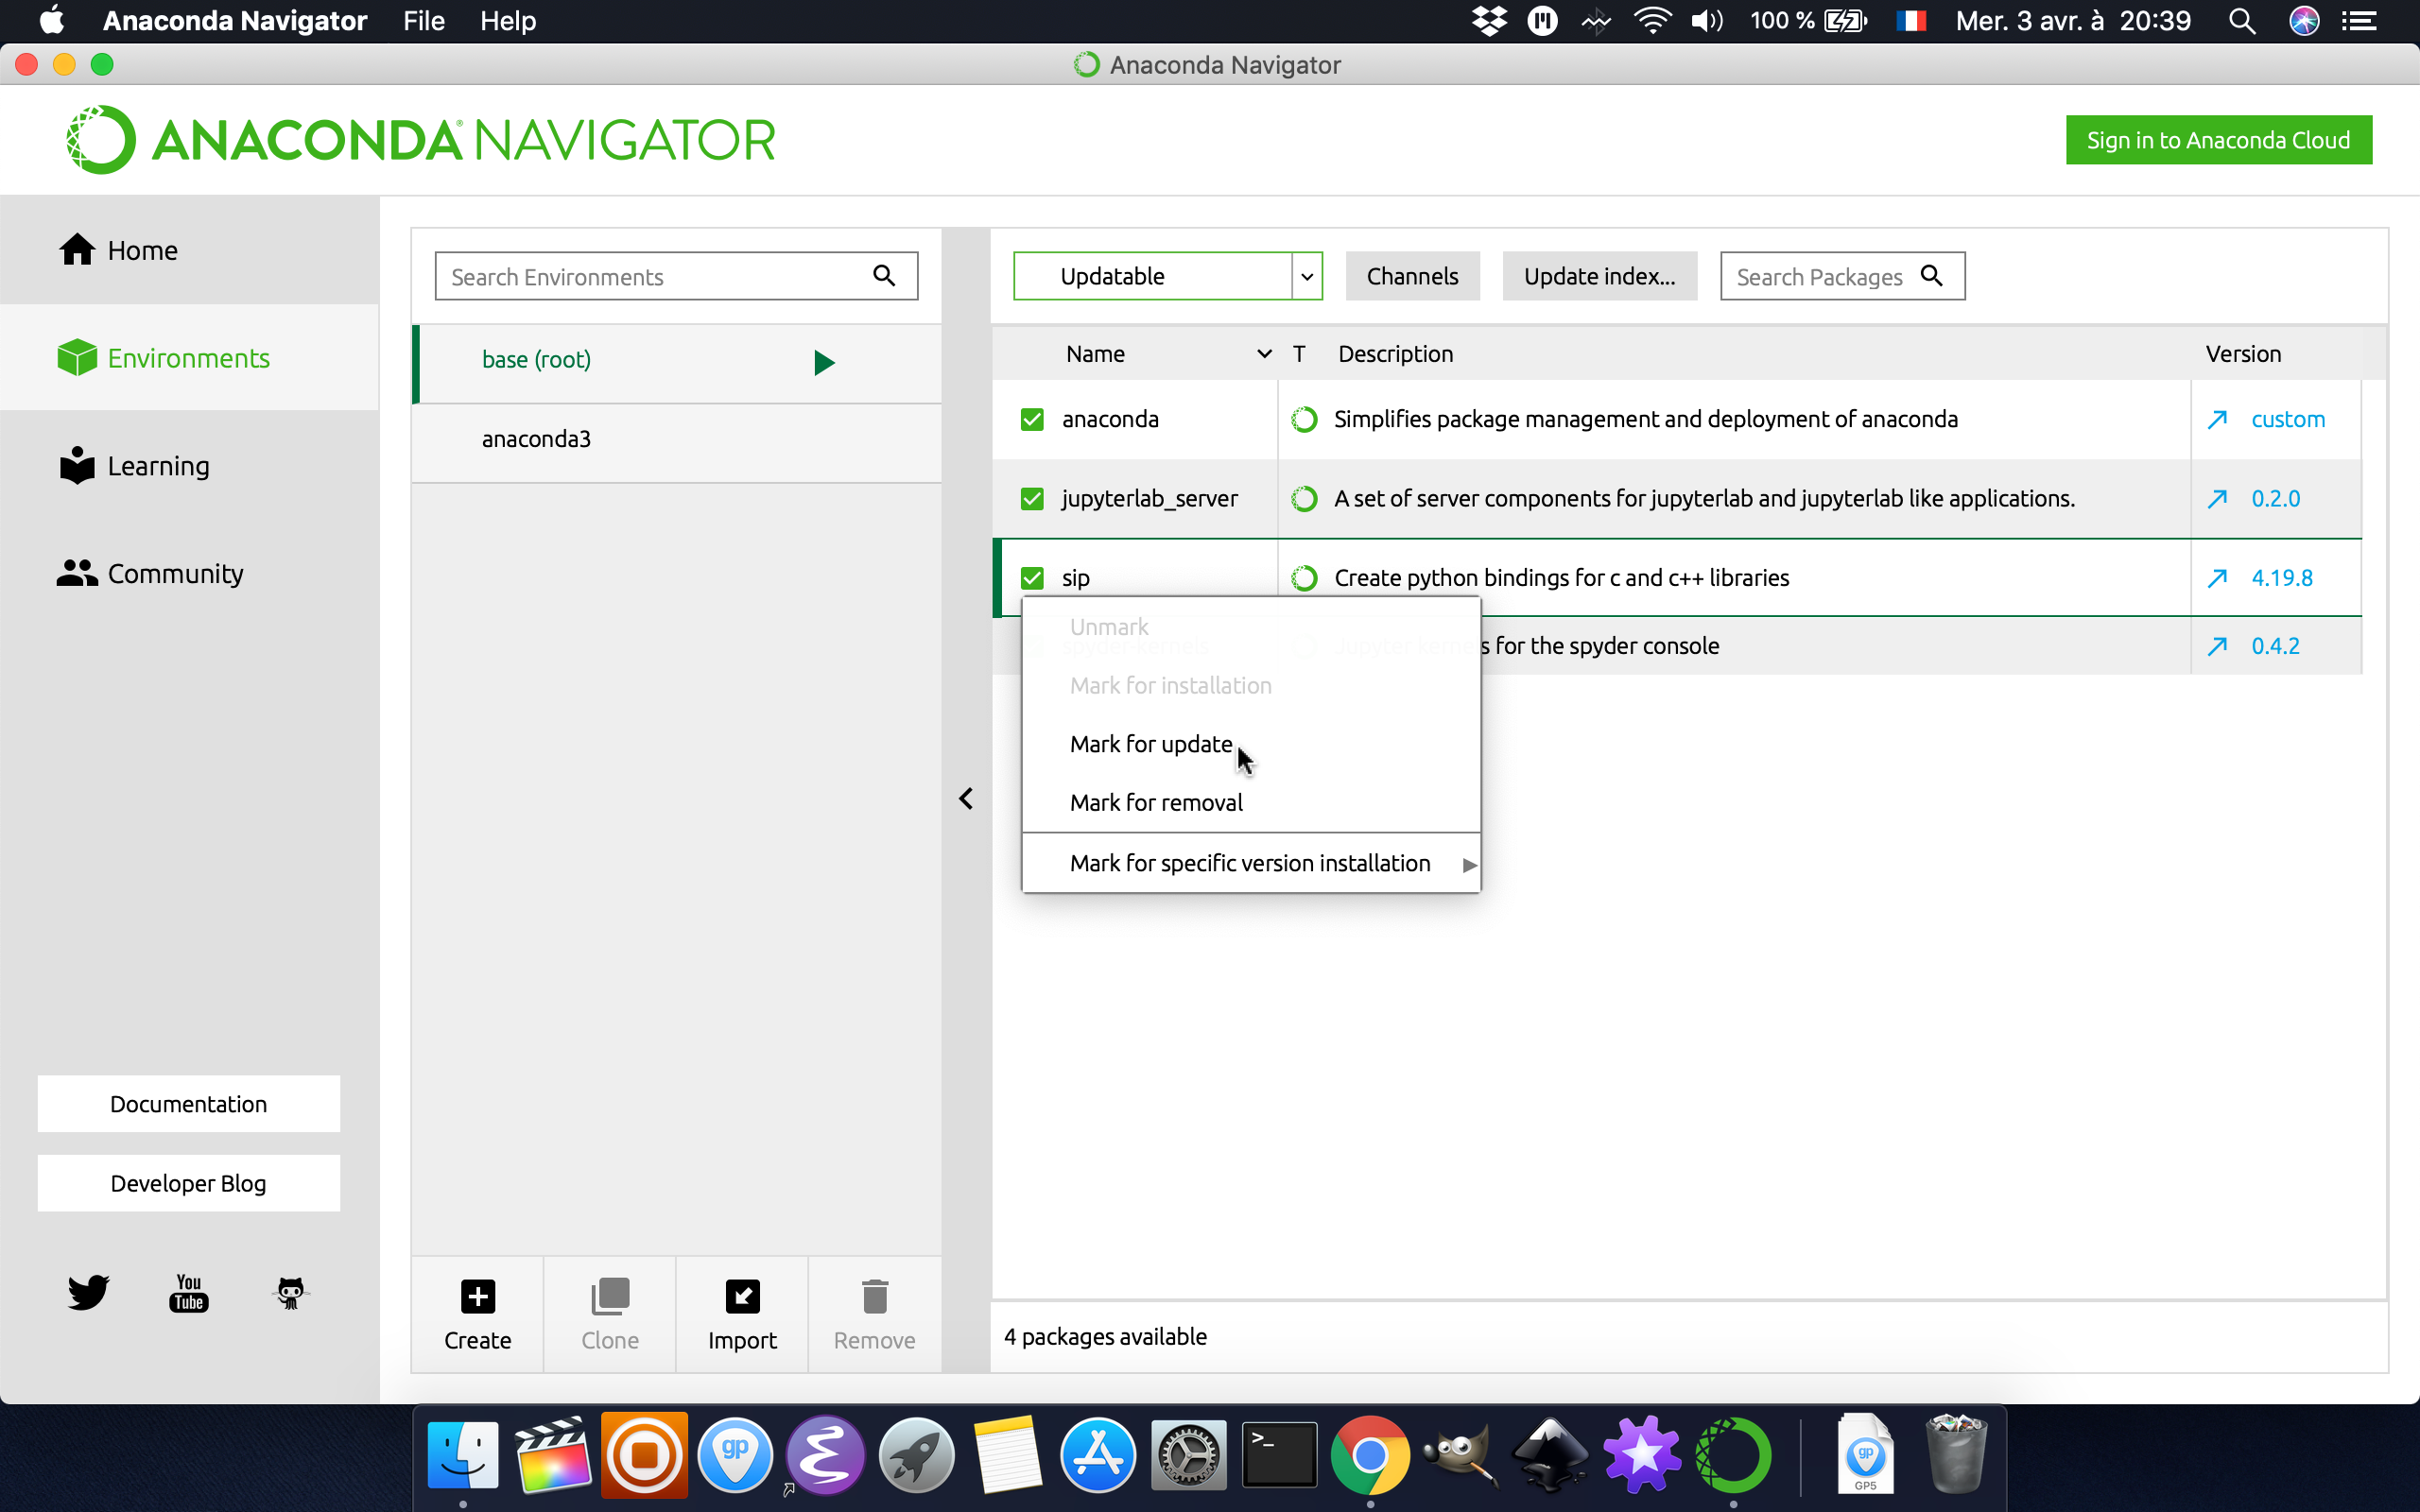
\includegraphics[height = .8\textheight]{anaconda-navigator-select-package-for-upgrade}
  \end{center}
\end{frame}

\begin{frame}{À l'aide de l'interface graphique : mise à jour}
  \begin{center}
    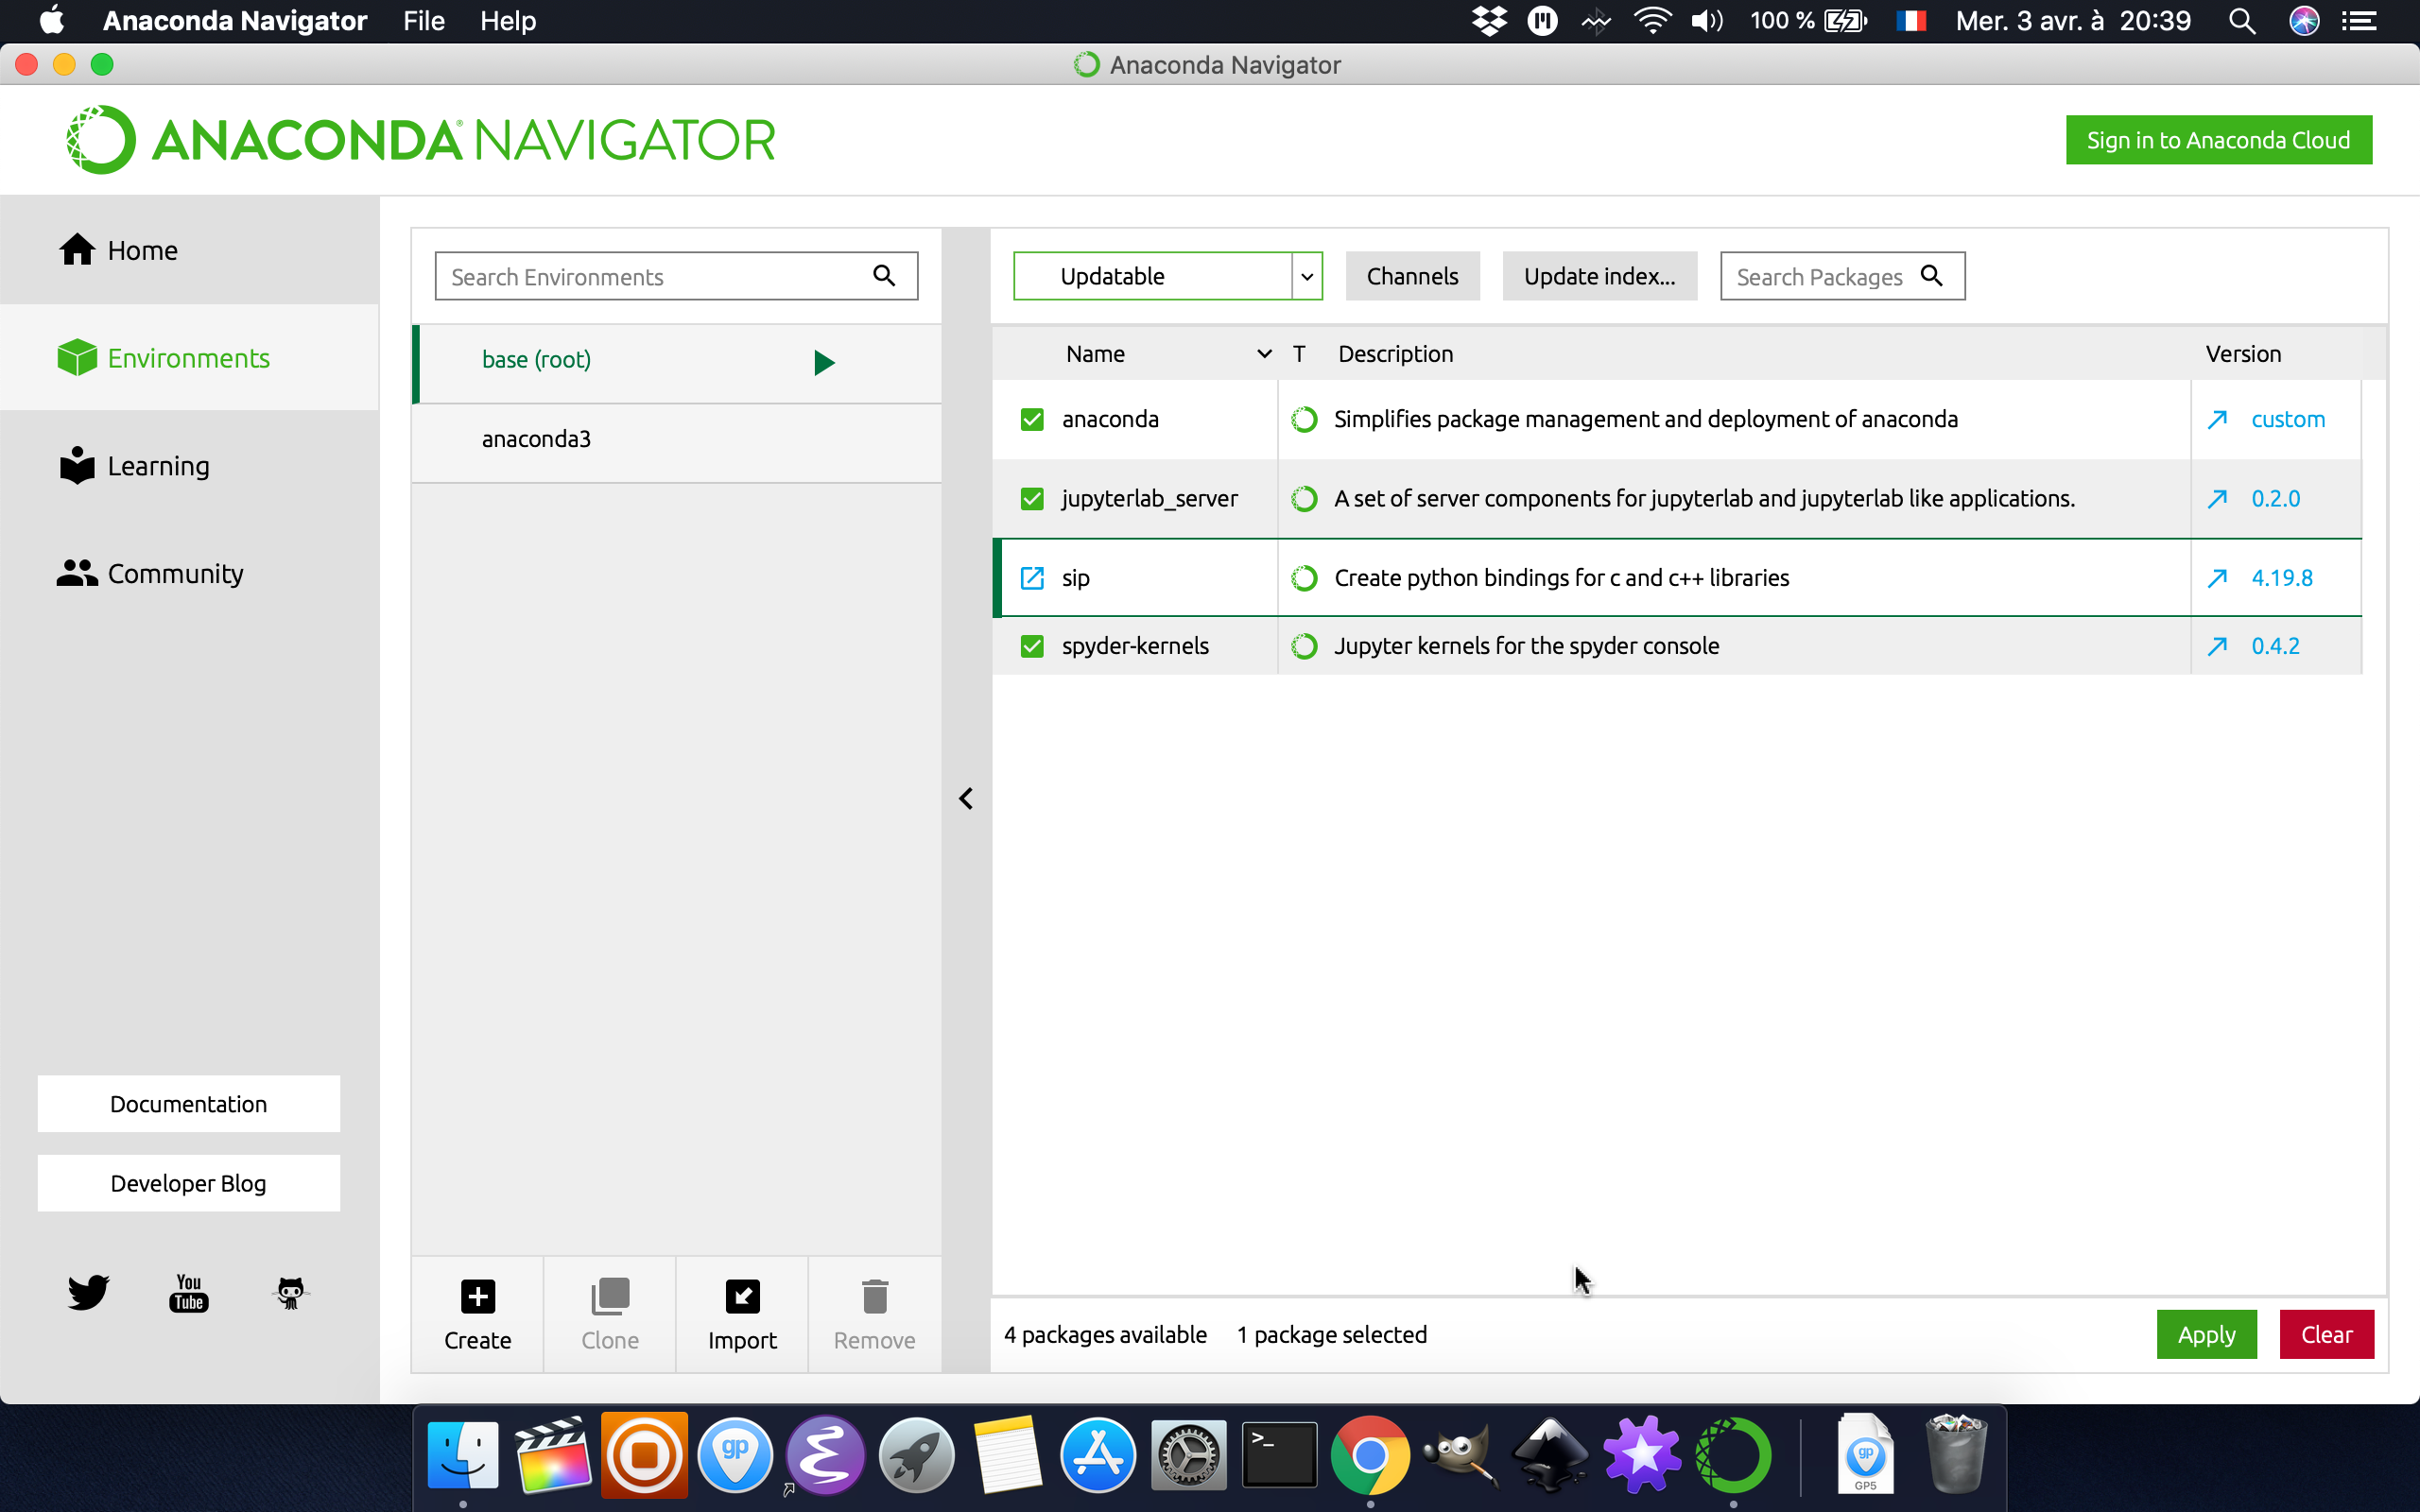
\includegraphics[height = .8\textheight]{anaconda-navigator-apply-upgrade}
  \end{center}
\end{frame}

\begin{frame}{À l'aide de l'interface graphique : installation d'un paquet}
  \begin{center}
    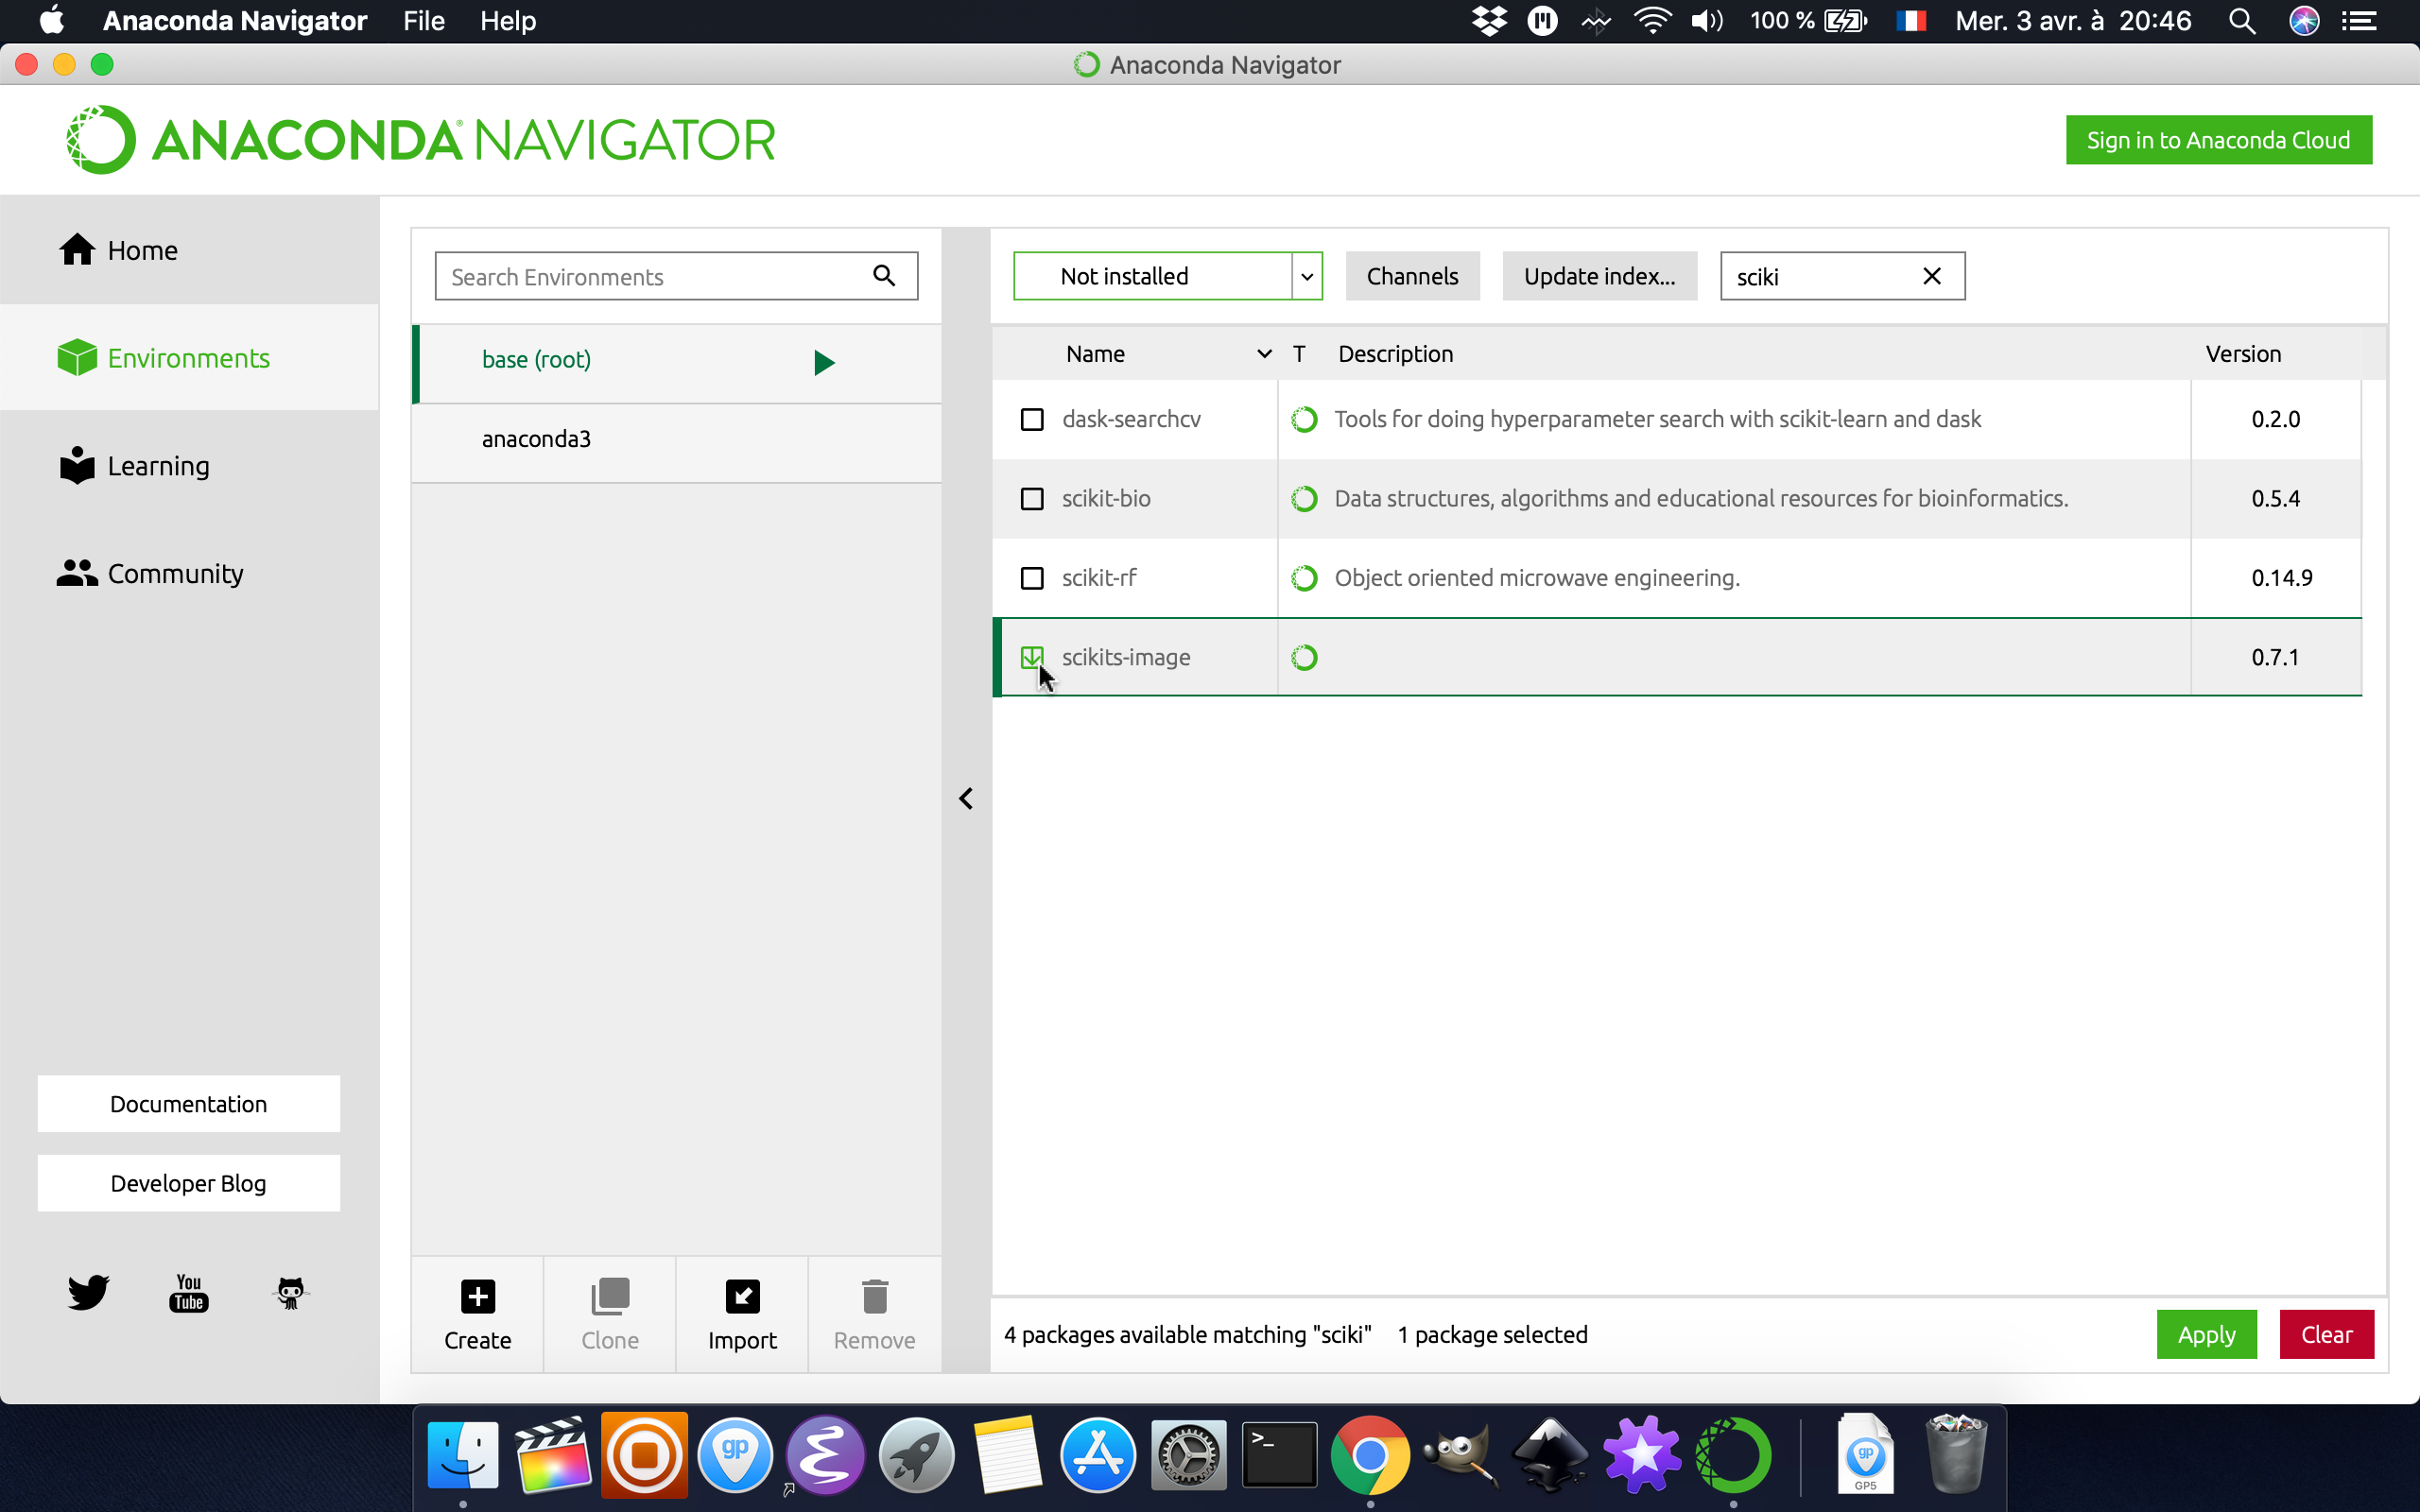
\includegraphics[height = .8\textheight]{anaconda-navigator-select-package-for-install}
  \end{center}
\end{frame}

\begin{frame}{En ligne de commande}
  \begin{center}
    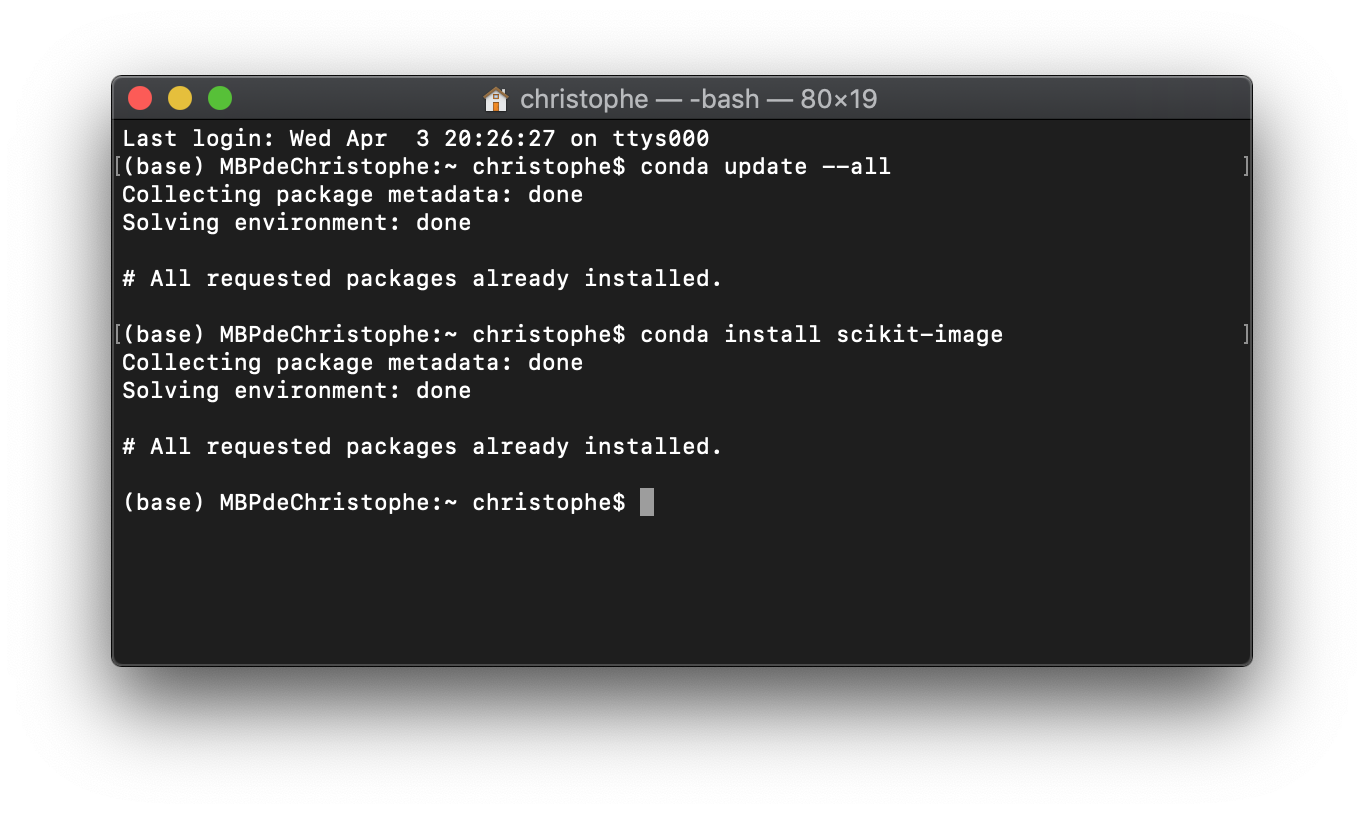
\includegraphics[height = .8\textheight]{conda-console-upgrade-install}
  \end{center}
\end{frame}

\section{Quelques façons d'utiliser Python}

\subsection{Éditeur et ligne de commande}

\begin{frame}{Un exemple \emph{hardcore} : éditeur et exécution dans la console}
  \begin{center}
    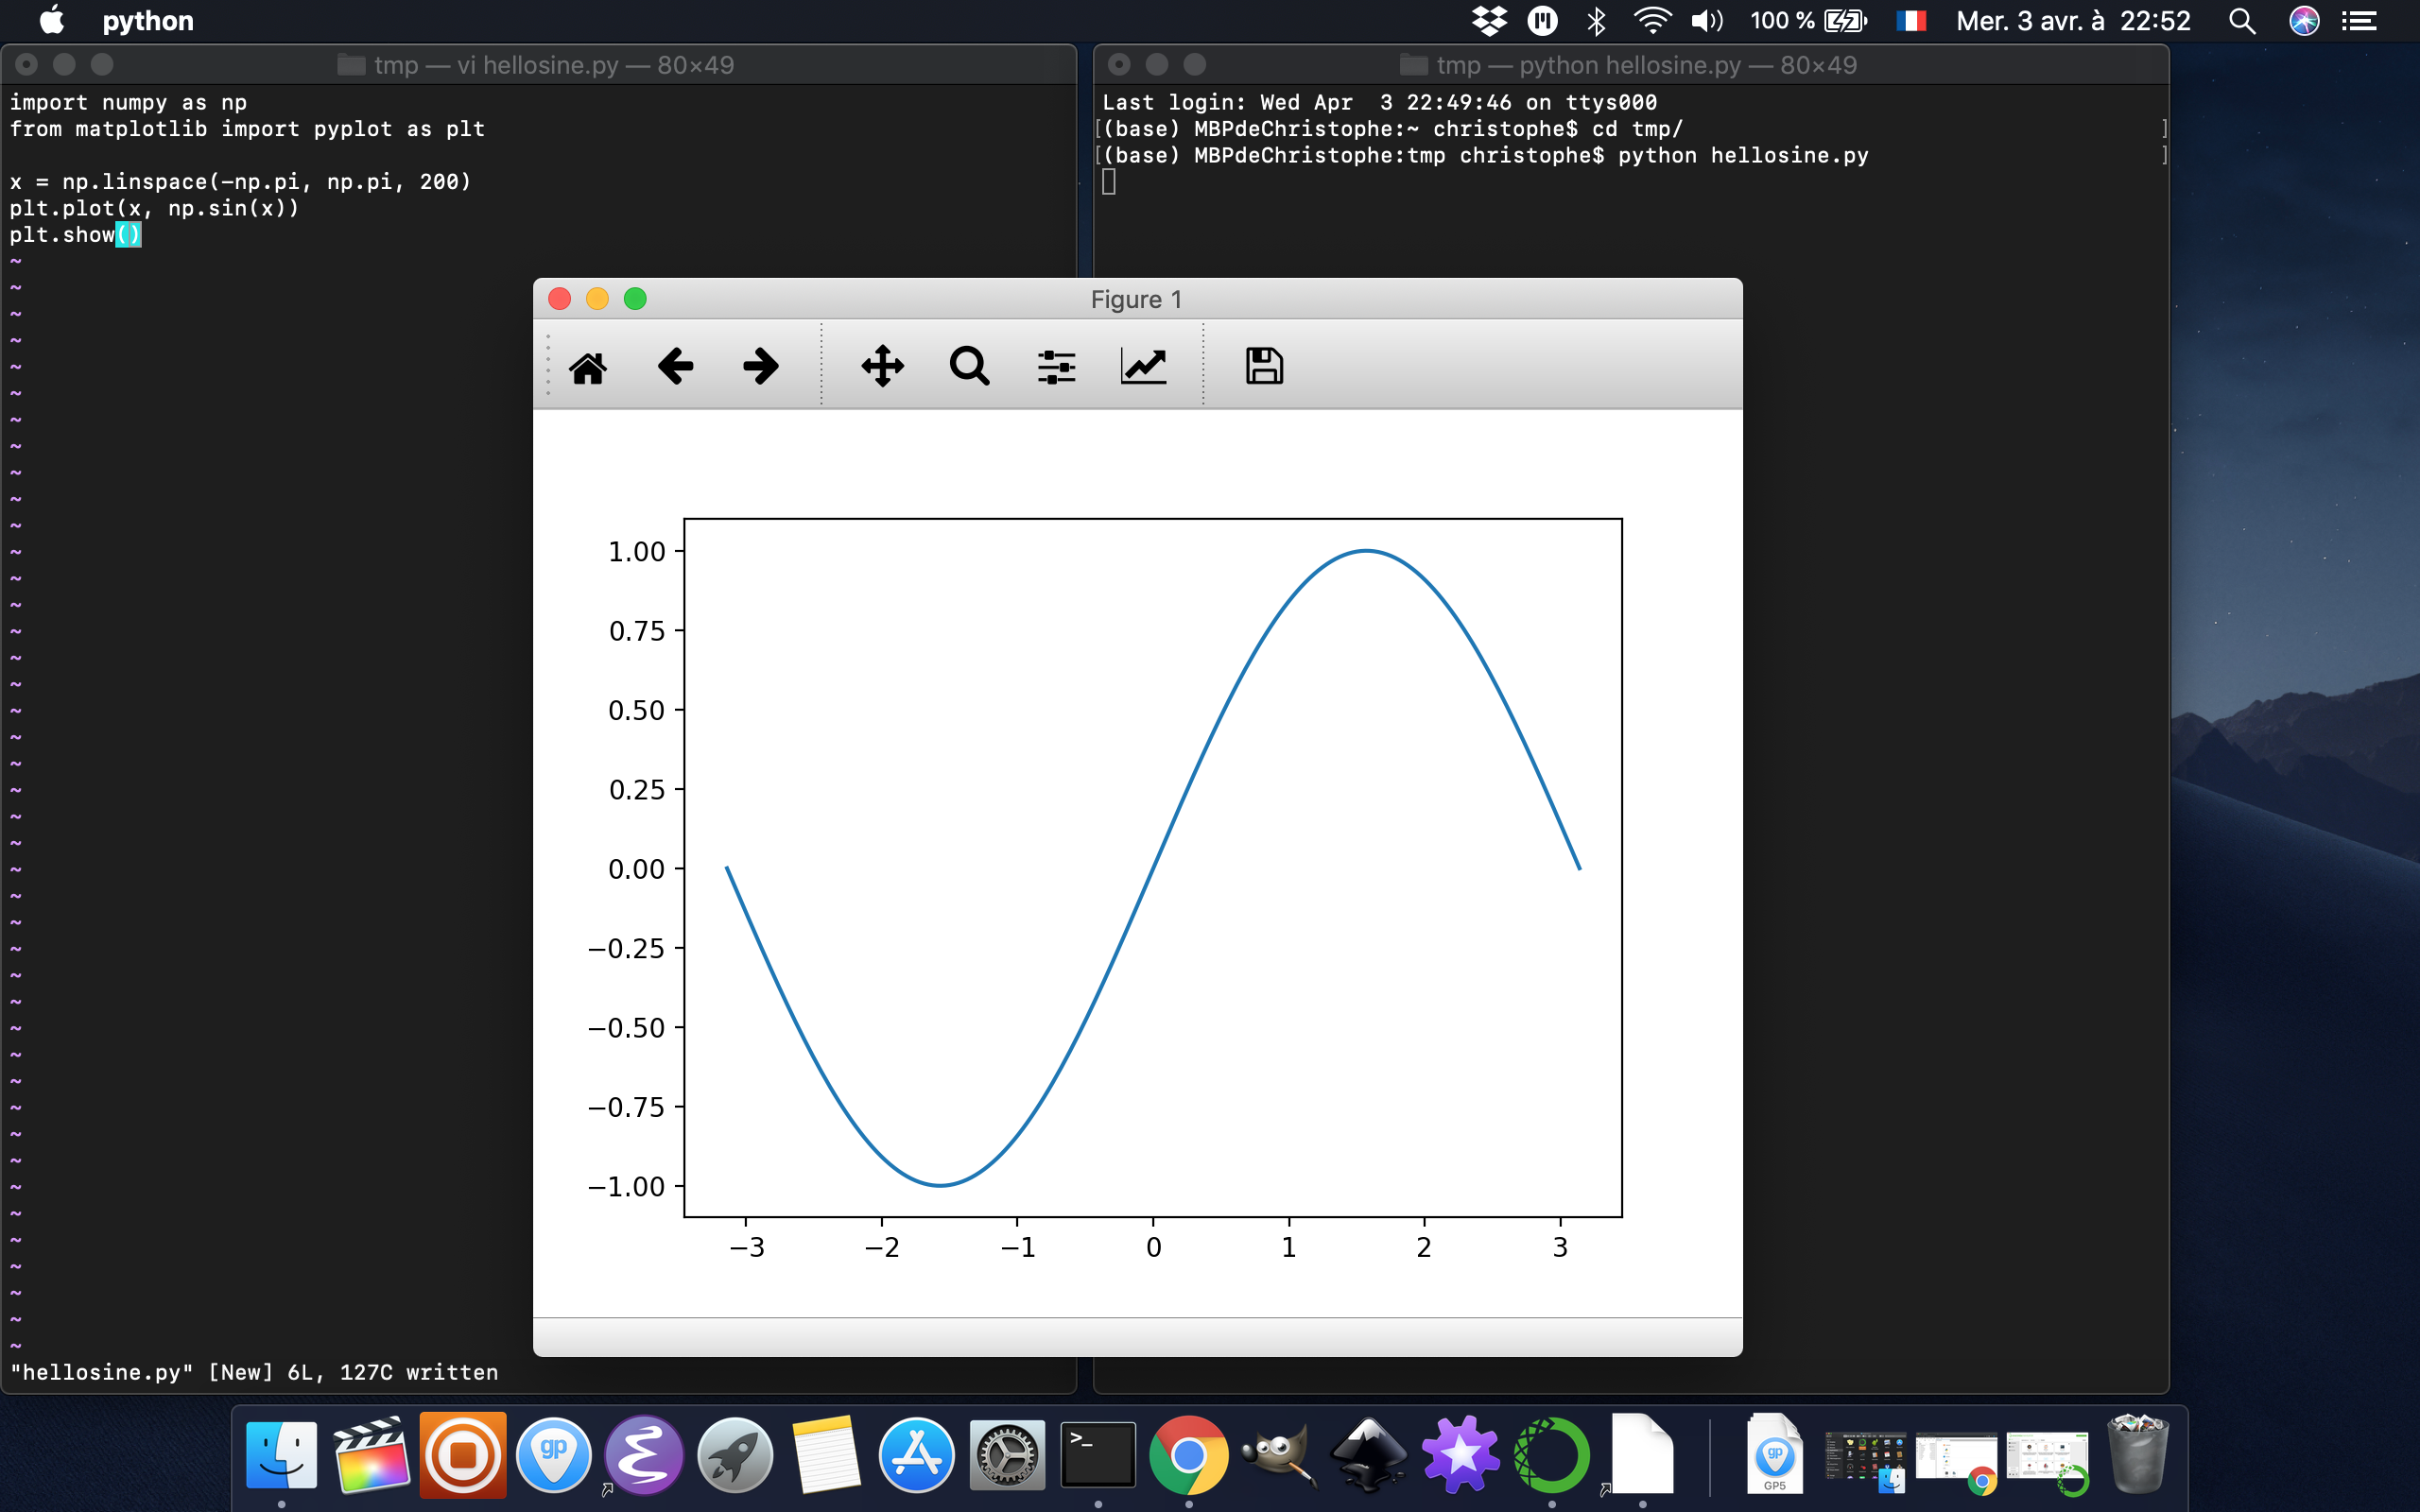
\includegraphics[height = .8\textheight]{vi-console-hellosine}
  \end{center}
\end{frame}

\subsection{IDE}

\begin{frame}{L'IDE d'Anaconda : spyder}
  \begin{center}
    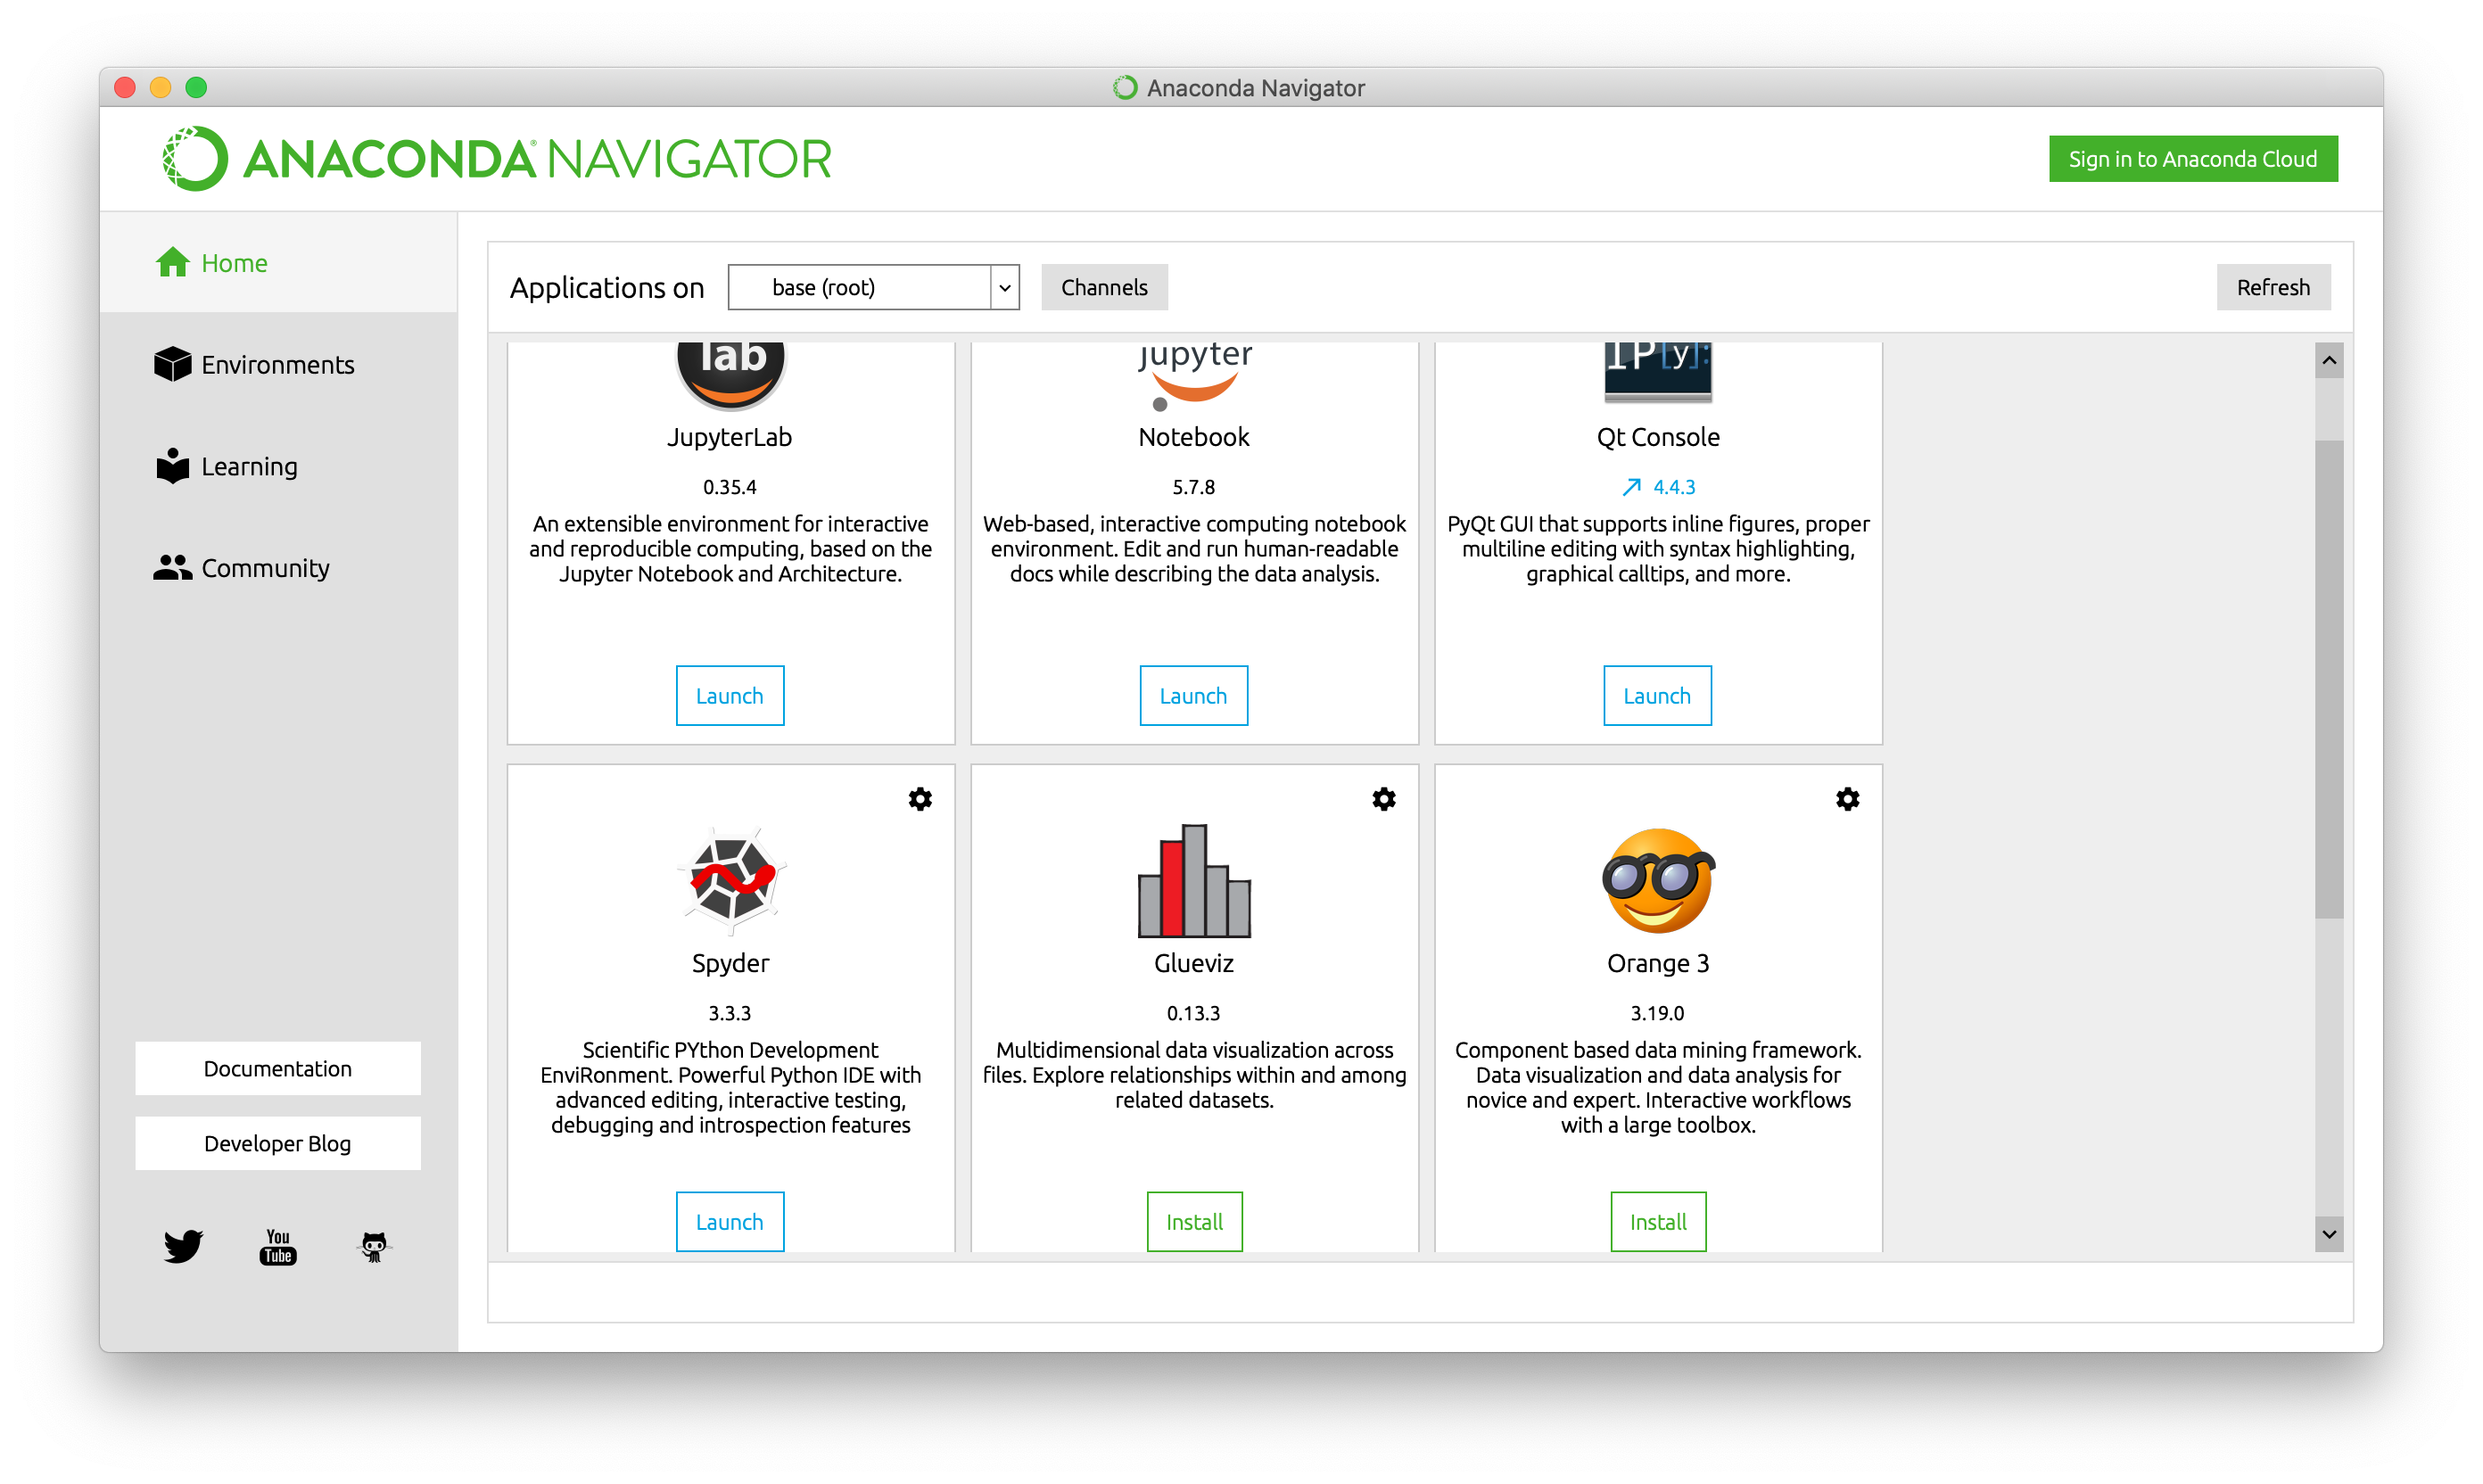
\includegraphics[height = .8\textheight]{anaconda-navigator-spyder-launch}
  \end{center}
\end{frame}

\begin{frame}{L'IDE d'Anaconda : spyder}
  \begin{center}
    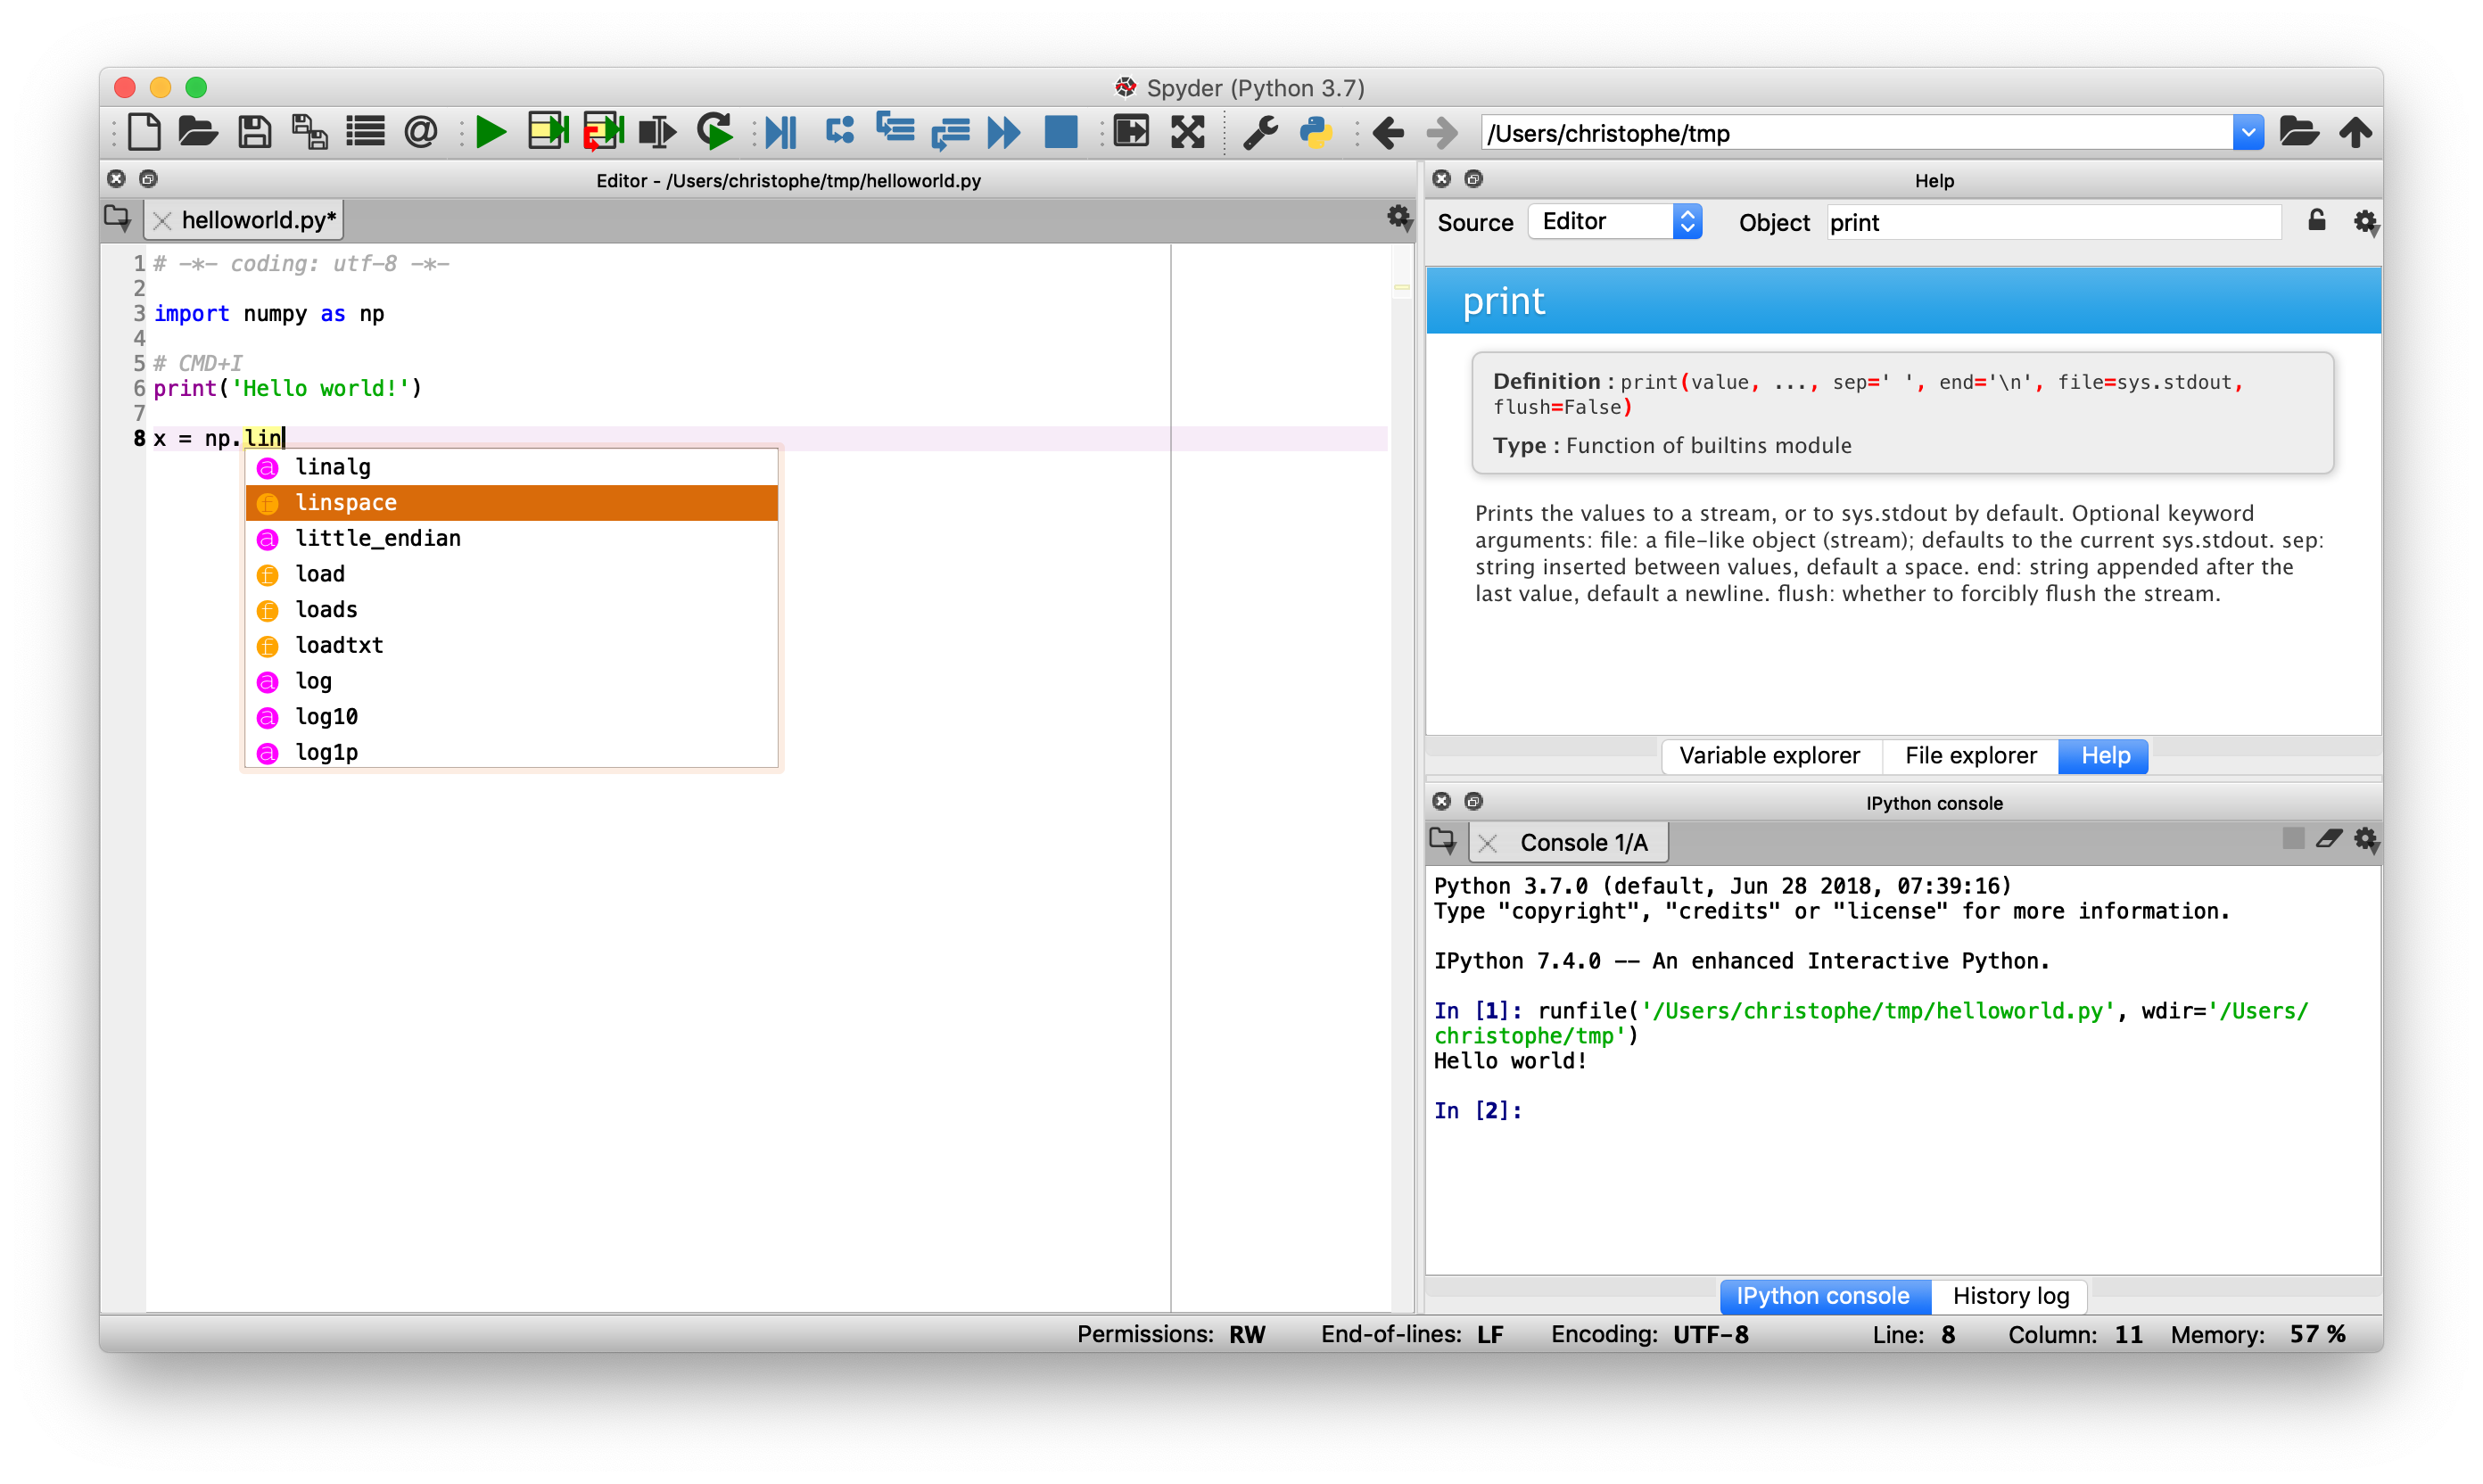
\includegraphics[height = .8\textheight]{spyder-help-completion}
  \end{center}
\end{frame}

\begin{frame}{L'IDE d'Anaconda : spyder}
  \begin{center}
    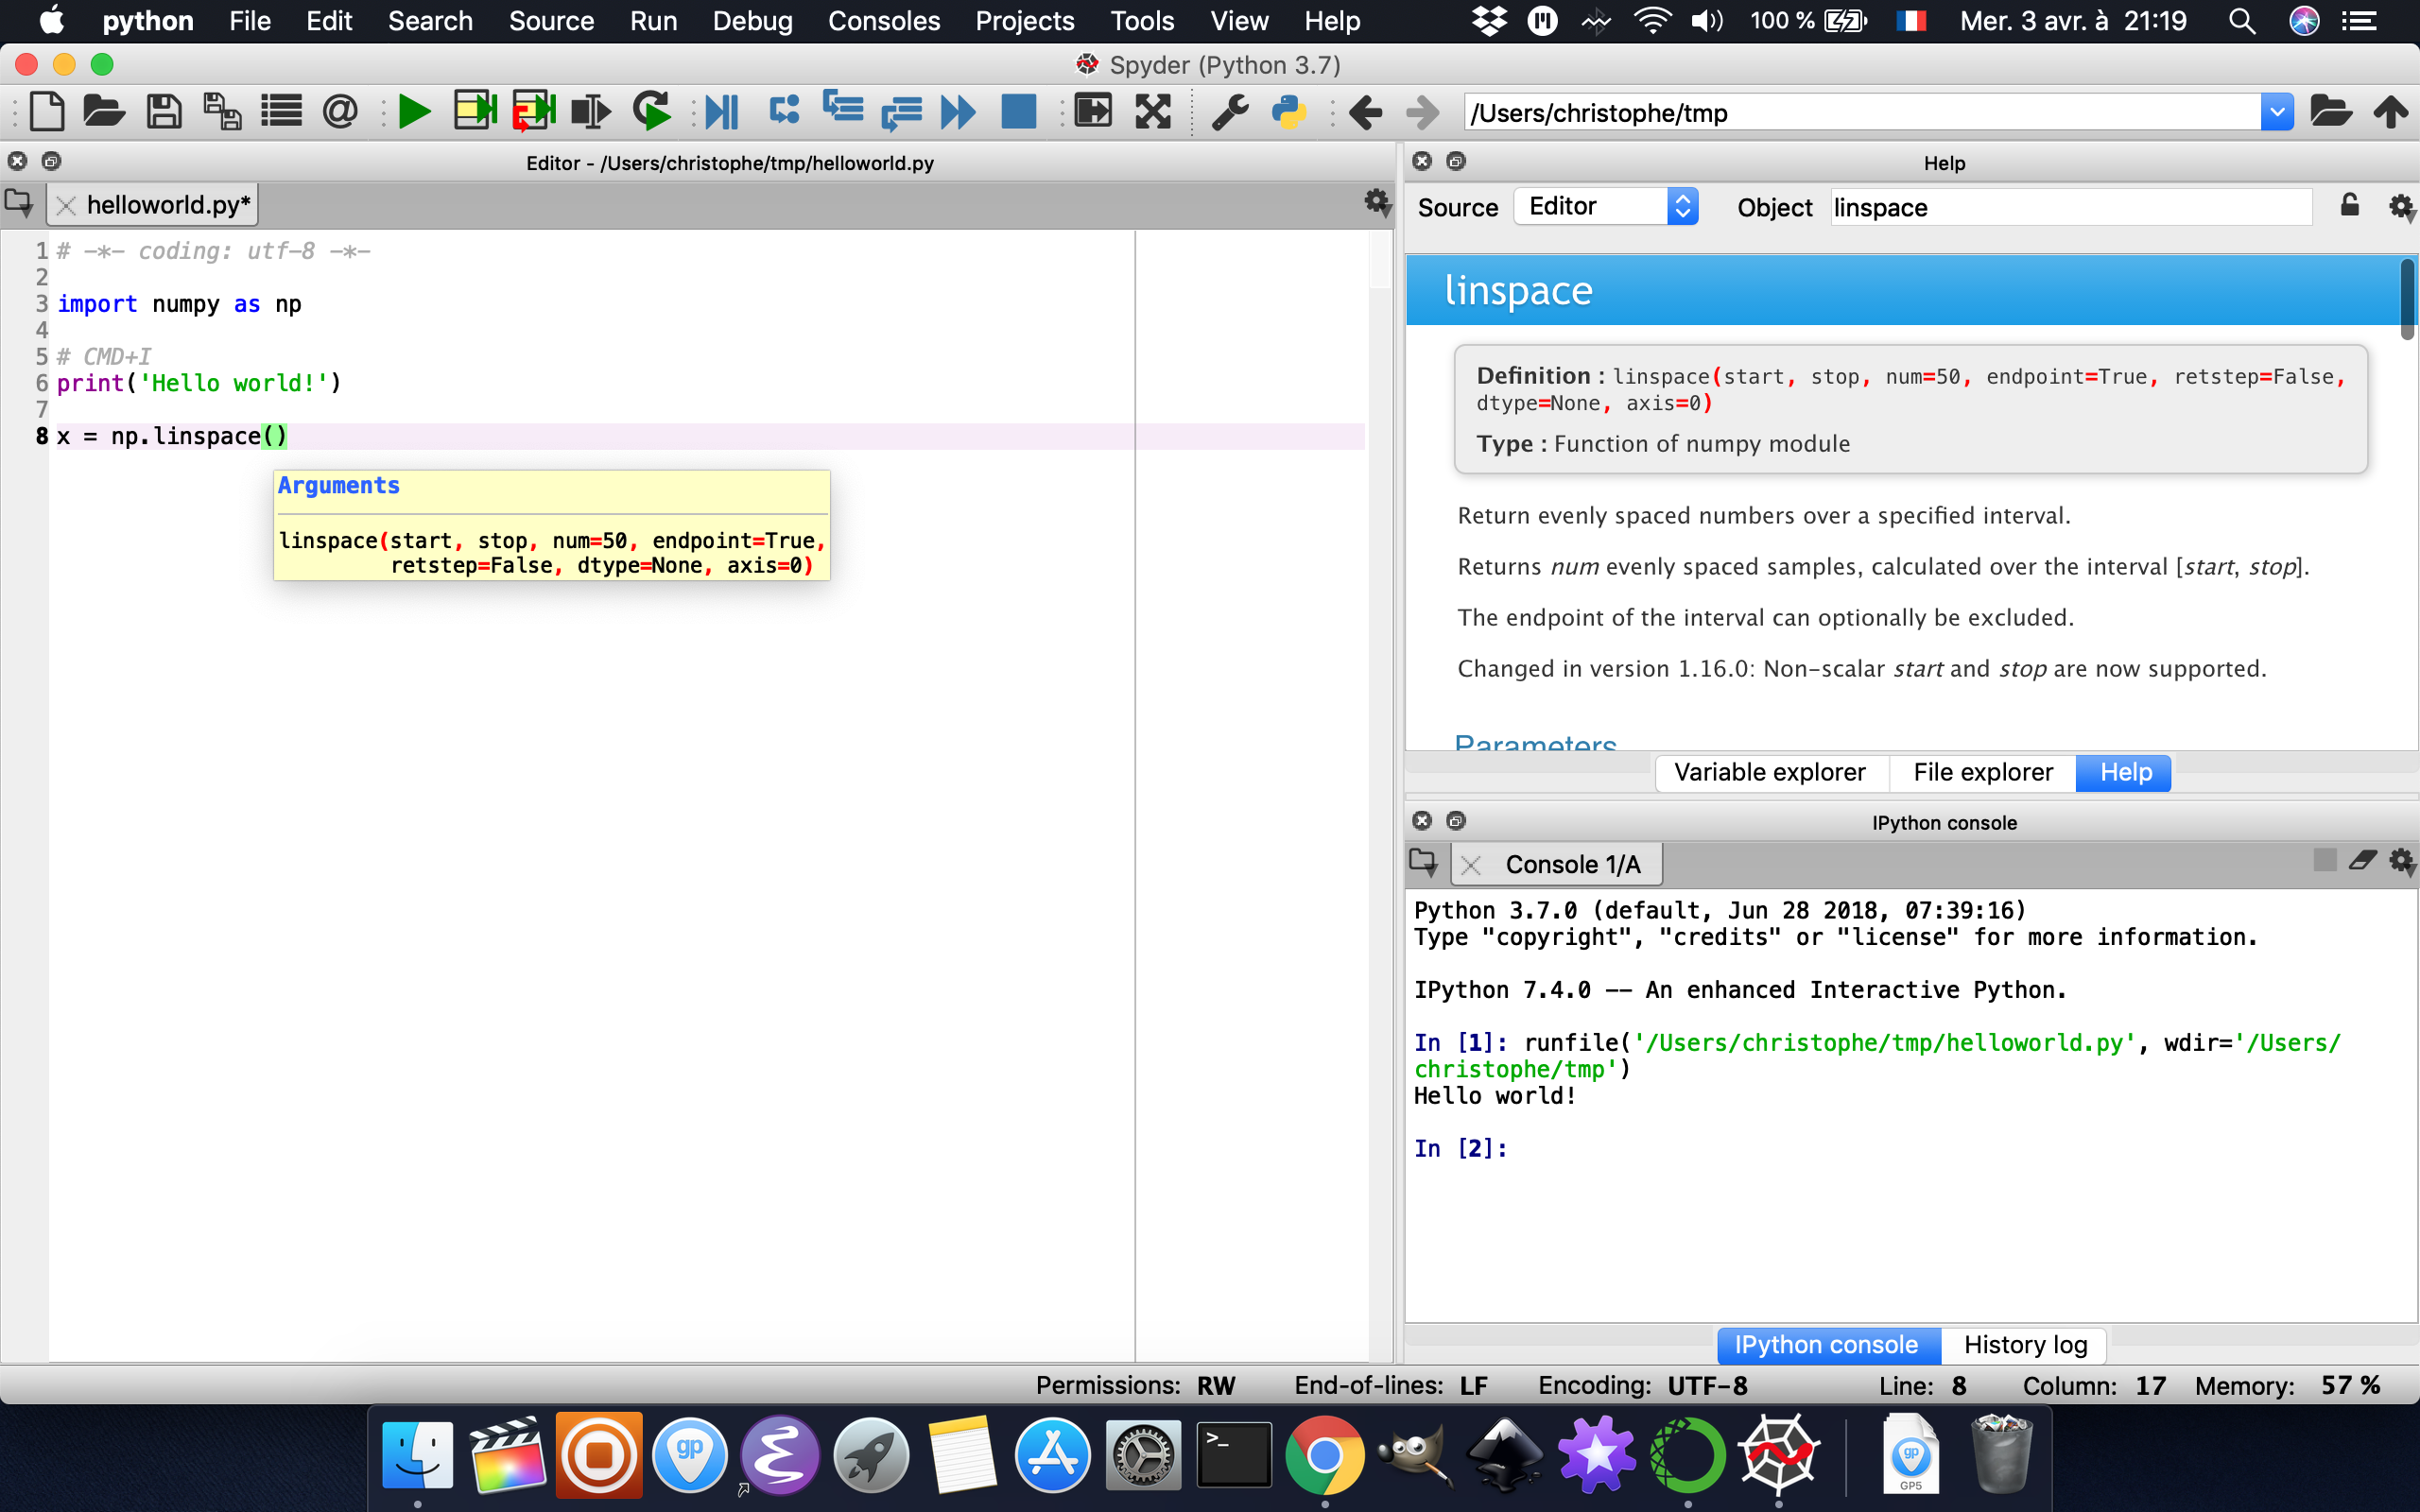
\includegraphics[height = .8\textheight]{spyder-help-info-popup}
  \end{center}
\end{frame}

\subsection{Dans le \emph{cloud} (dans le navigateur)}

\begin{frame}
  \begin{Conseil}
    C'est la solution de dépannage qui peut fonctionner sur n'\alert{importe quel ordinateur} ou \alert{smartphone} disposant d'une connexion internet d'un navigateur \alert{récent}.
  \end{Conseil}
\end{frame}

\begin{frame}{CS50 \emph{sandbox}}
  \begin{center}
    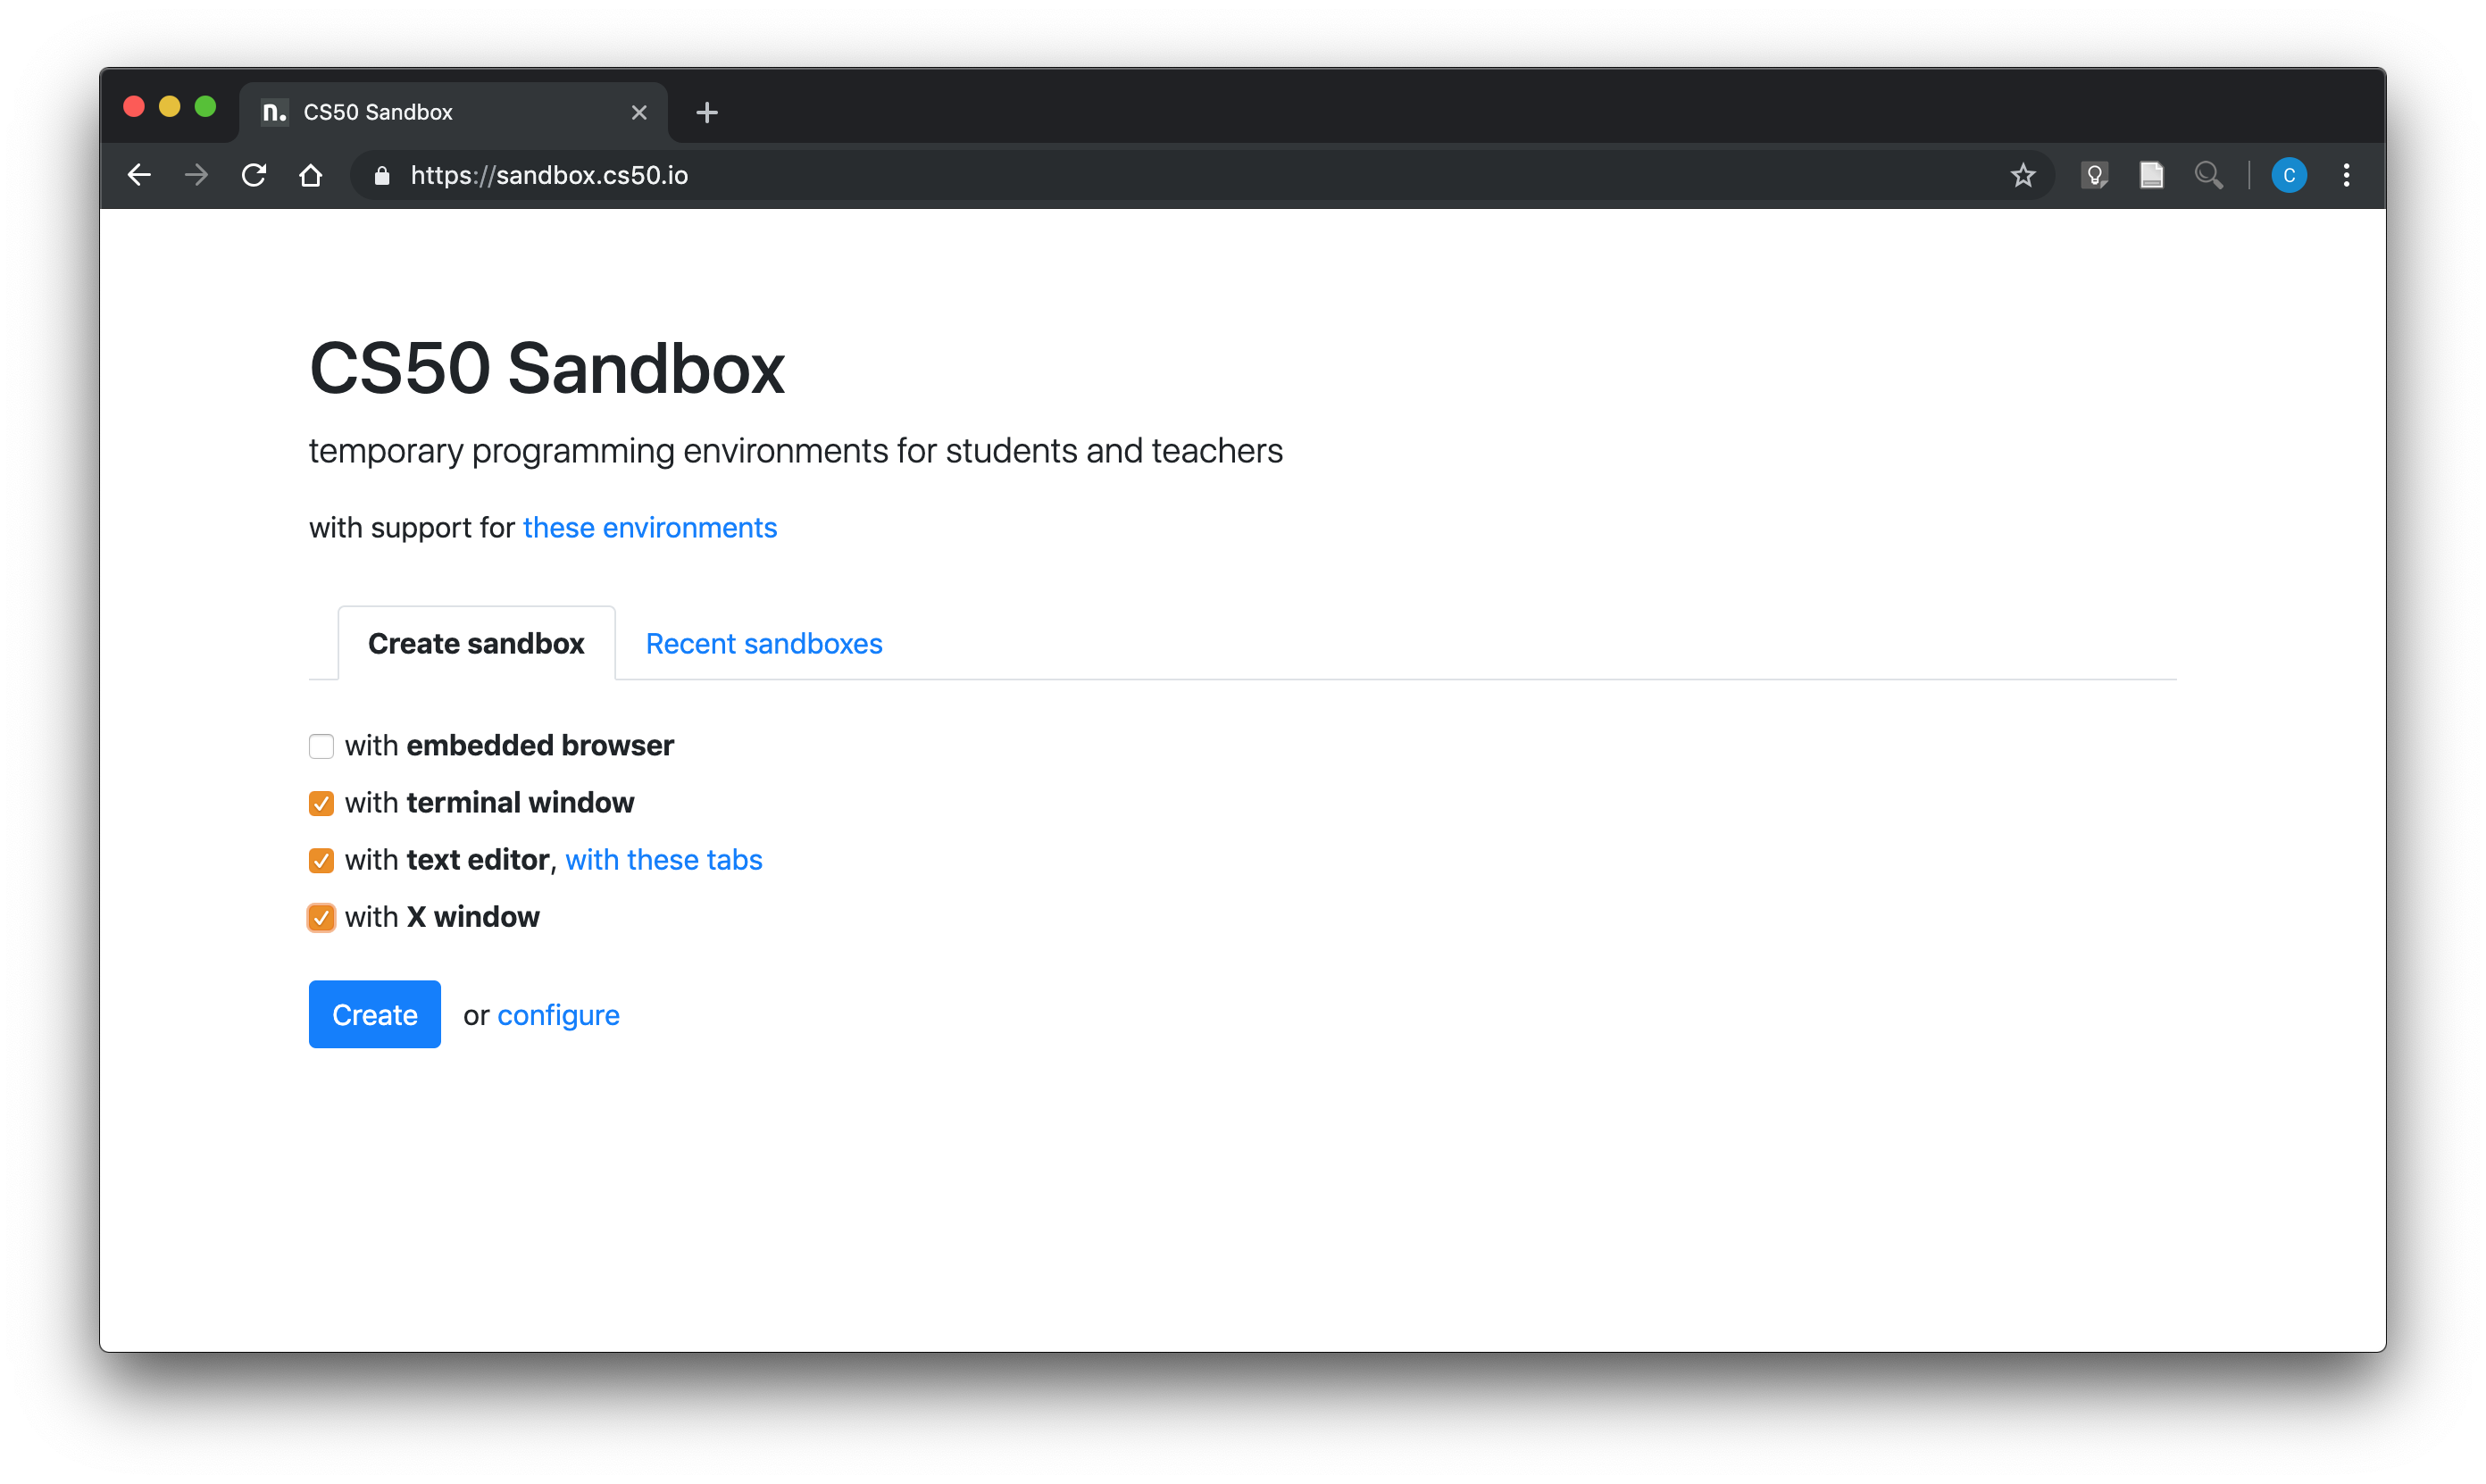
\includegraphics[height = .8\textheight]{cs50-create-page}
  \end{center}
\end{frame}

\begin{frame}{CS50 \emph{sandbox}}
  \begin{center}
    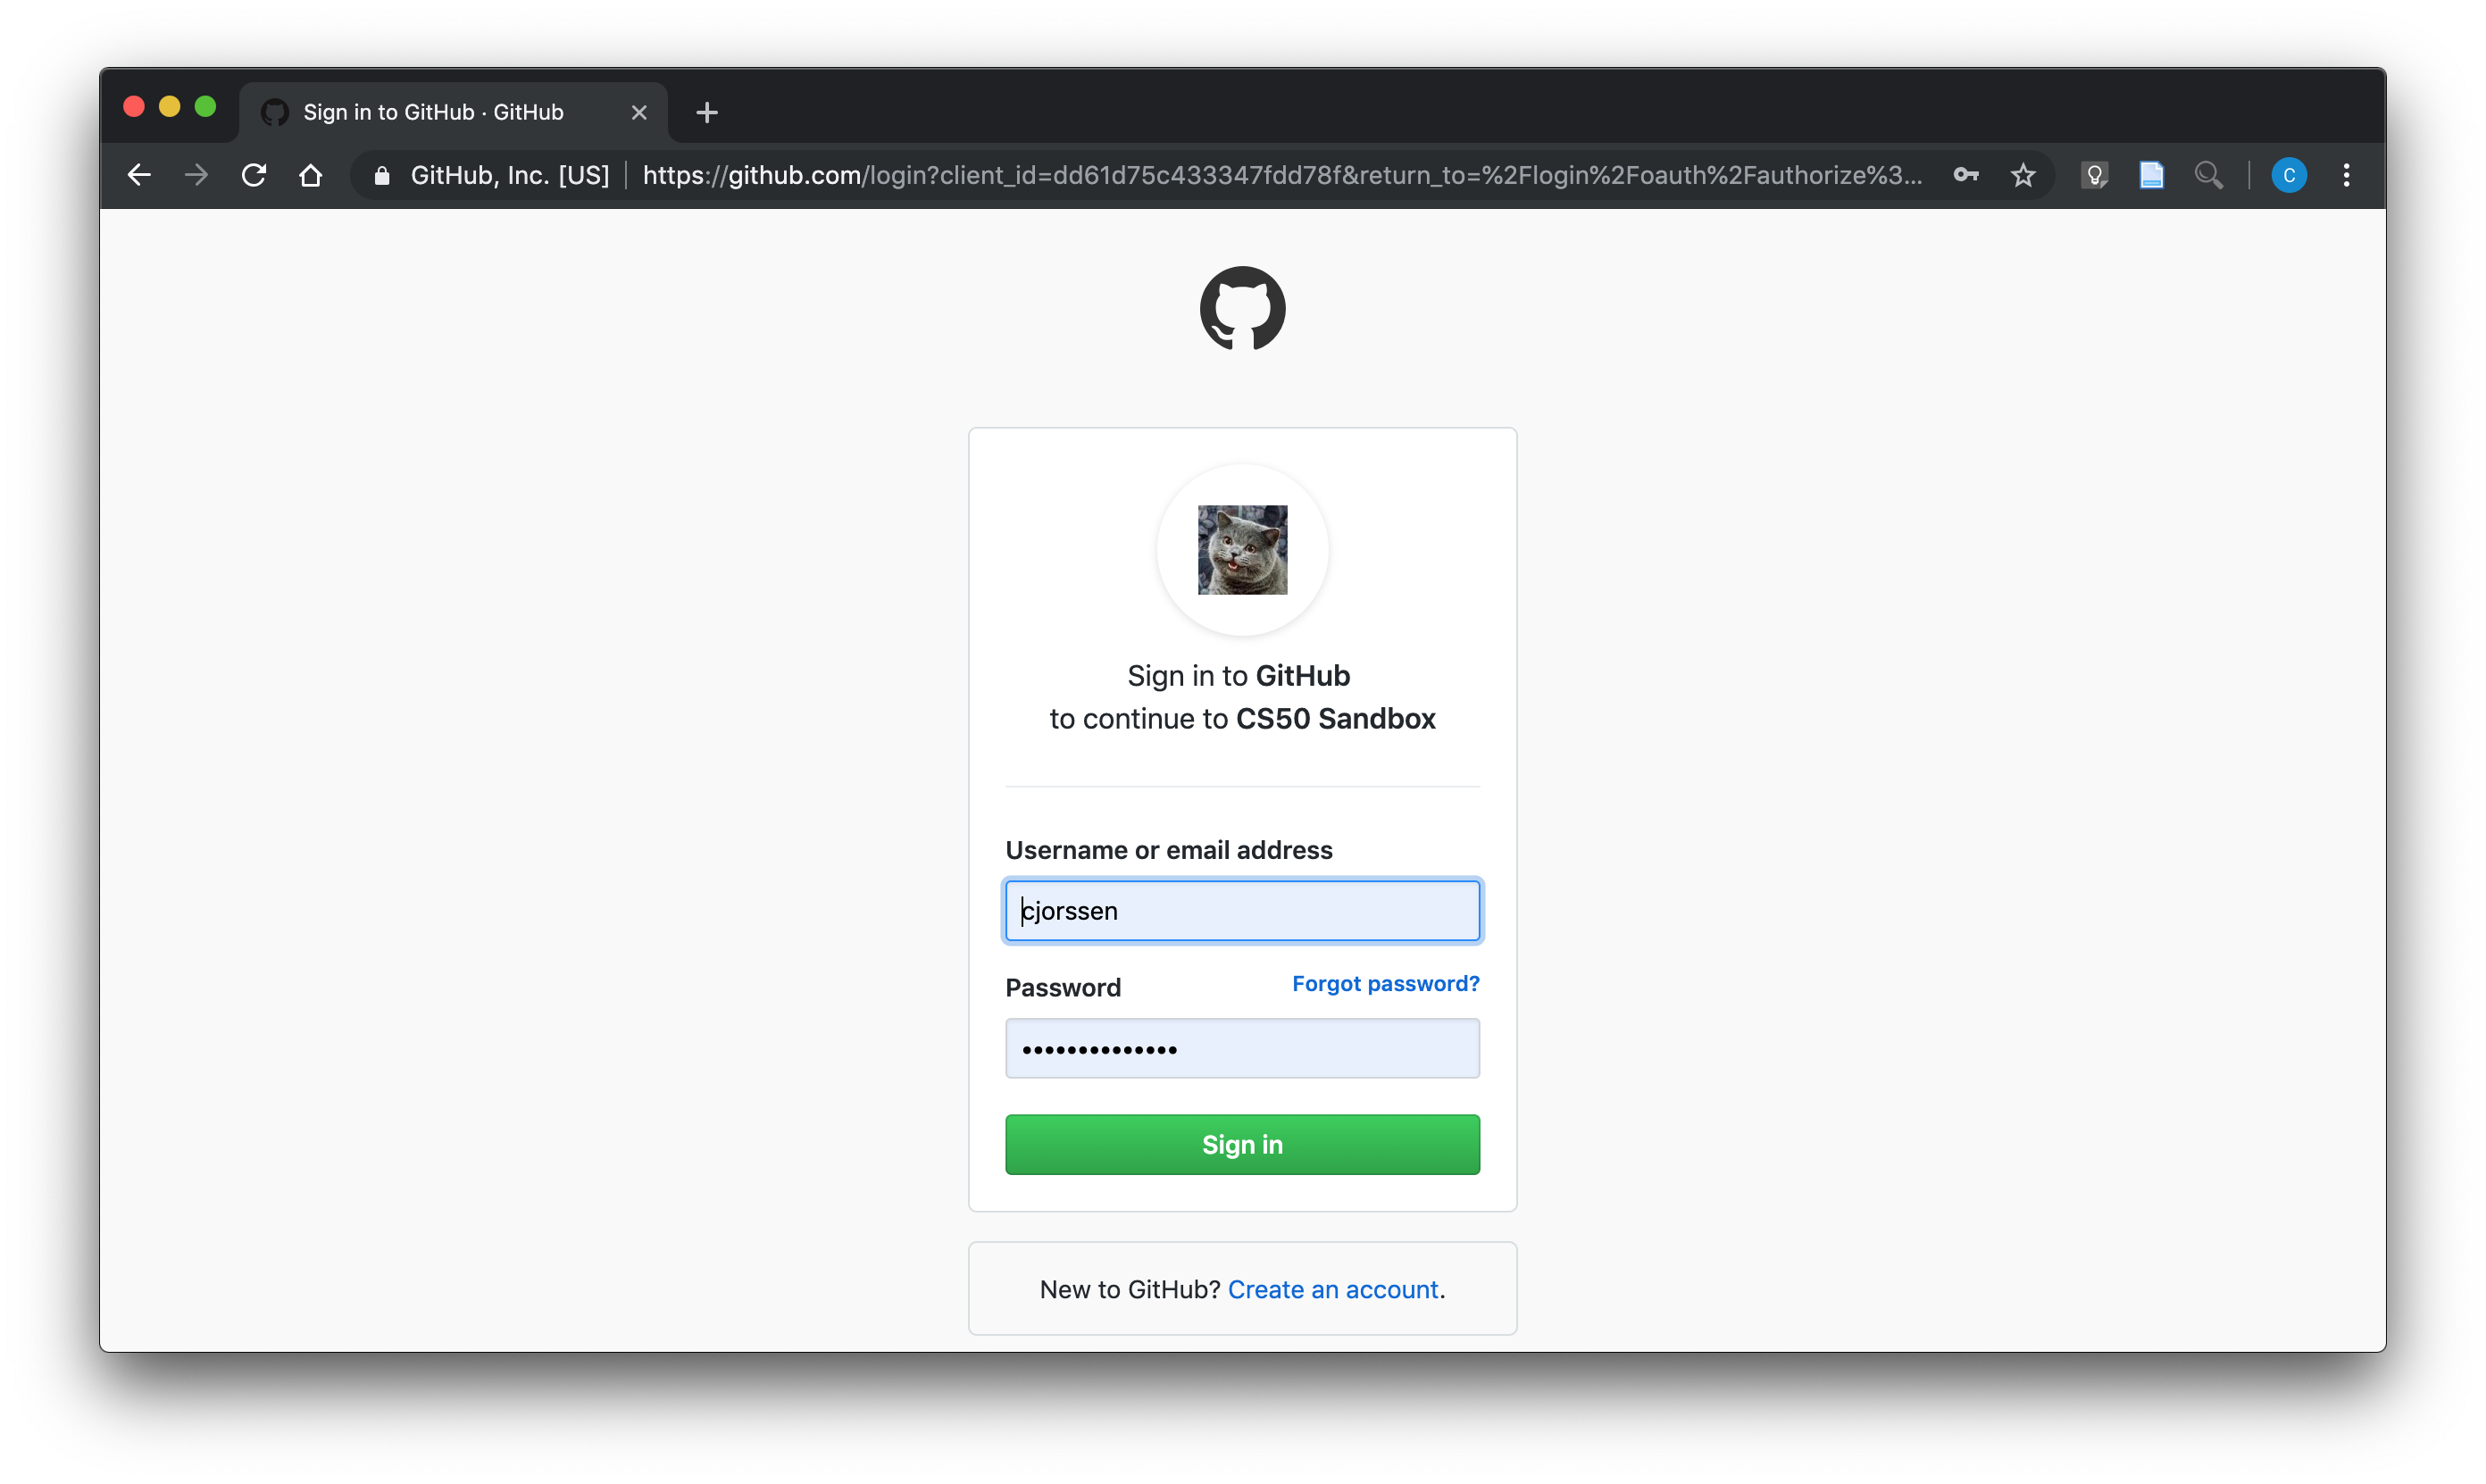
\includegraphics[height = .8\textheight]{cs50-github}
  \end{center}
\end{frame}

\begin{frame}{CS50 \emph{sandbox}}
  \begin{center}
    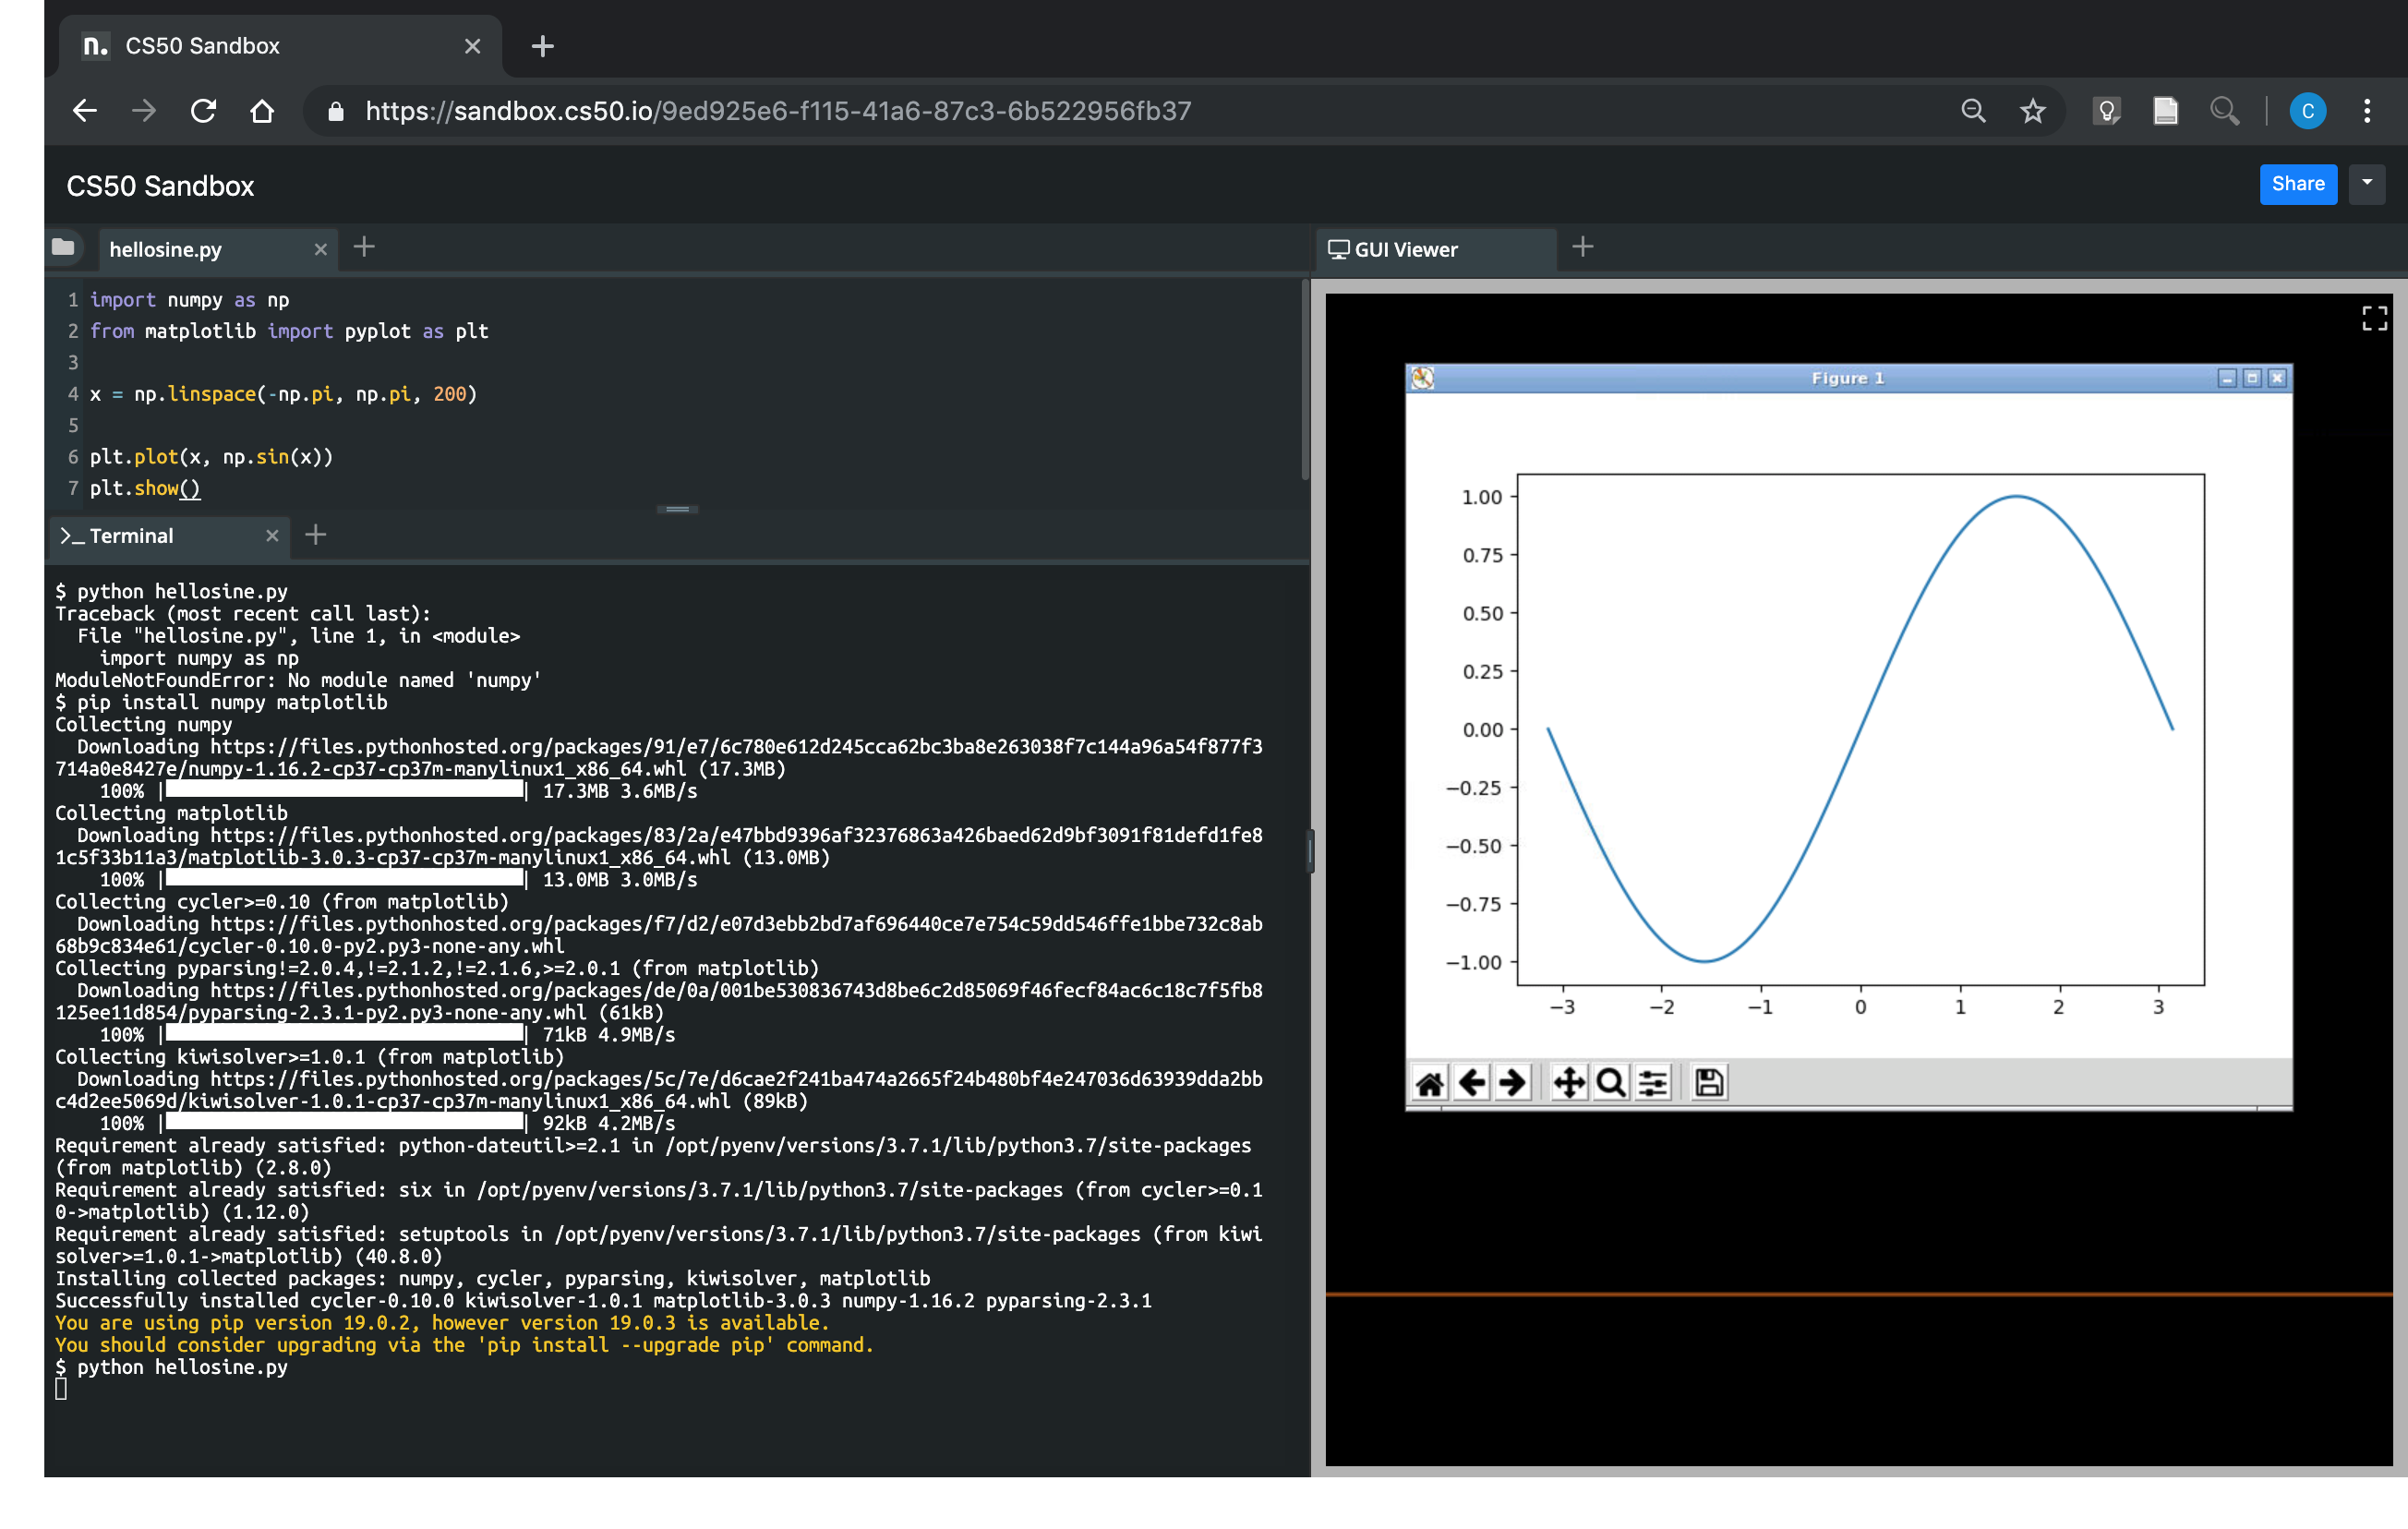
\includegraphics[height = .8\textheight]{cs50-hellosine}
  \end{center}
\end{frame}

\begin{frame}{\url{repl.it}}
  \begin{center}
    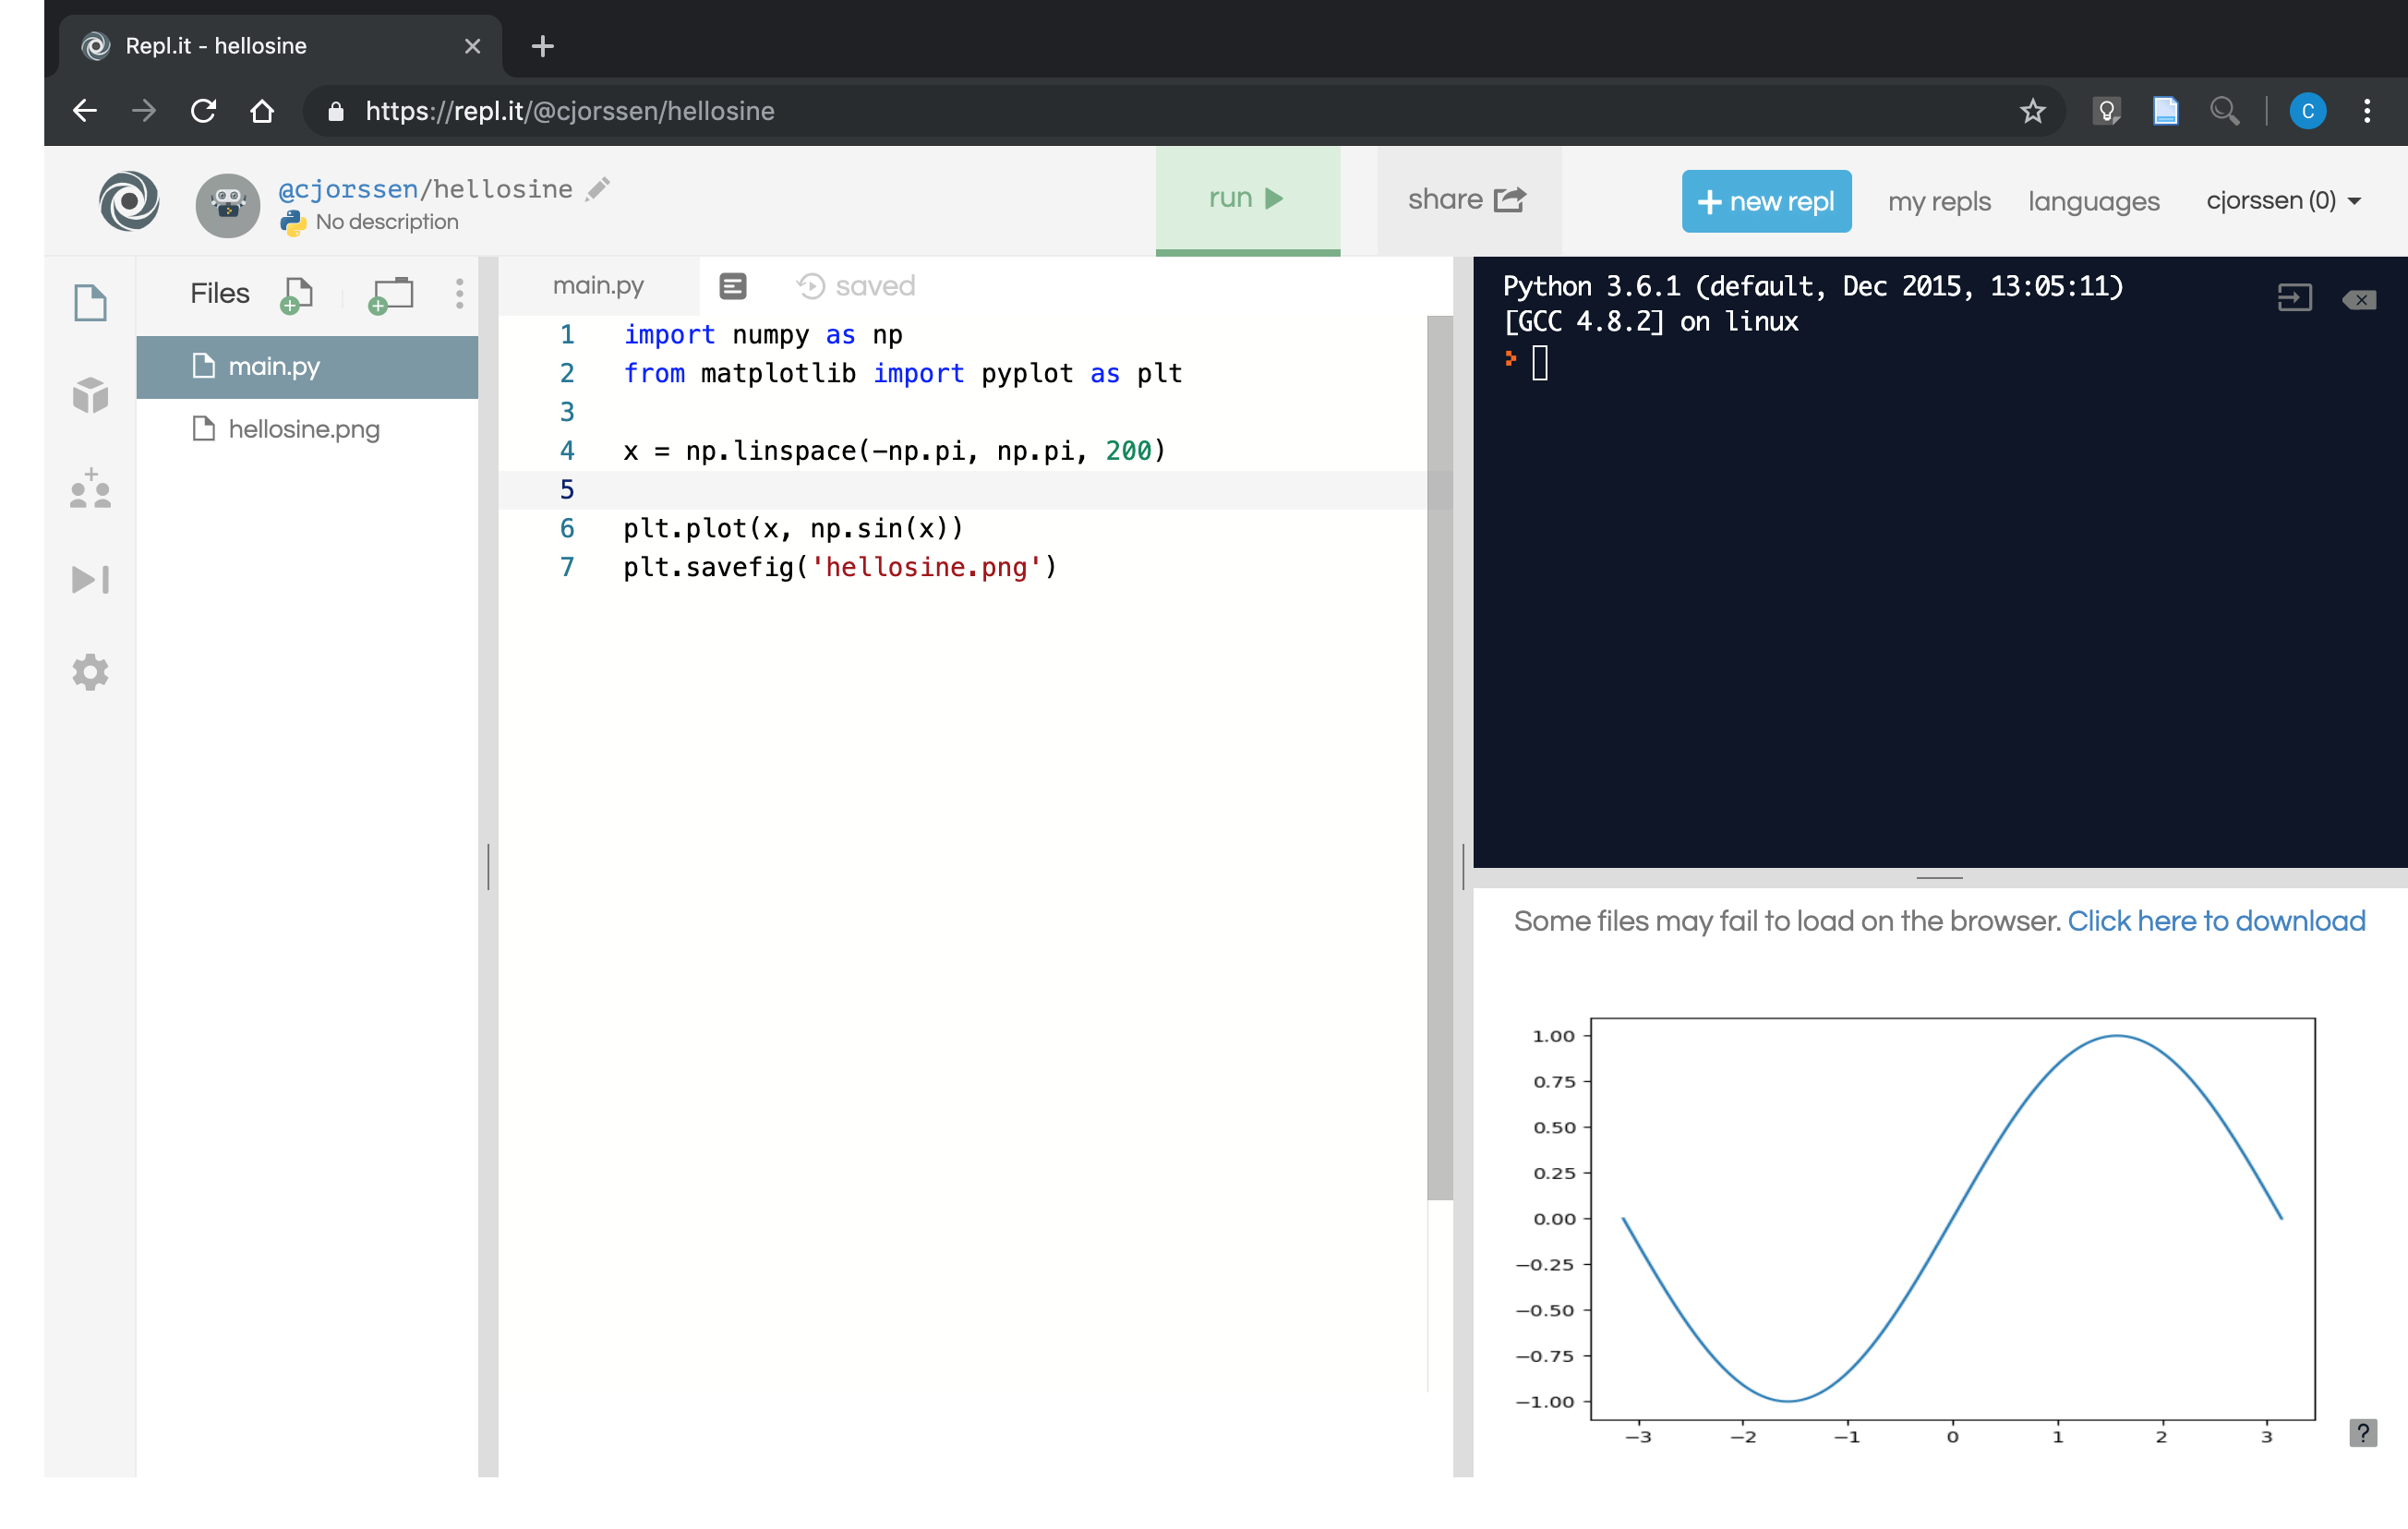
\includegraphics[height = .8\textheight]{replit-hellosine}
  \end{center}
\end{frame}

\subsection{Avec des \emph{notebooks}}

\begin{frame}
  \begin{Definition}
    Un \emph{notebook} est une page \texttt{html} :
    \begin{itemize}
    \item qui peut mélanger :
      \begin{itemize}
      \item du texte (mis en forme) ;
      \item du \LaTeX{} (rendu) ;
      \item du code Python et son exécution (y compris des représentations graphiques) ;
      \item des vidéos ou de l'audio ;
      \item etc ;
      \end{itemize}
    \item totalement éditable dans le navigateur et dynamique (à condition de disposer d'un serveur jupyter).
    \end{itemize}
  \end{Definition}
\end{frame}

\begin{frame}
  \begin{BonASavoir}
    C'est une méthode qui fonctionne :
    \begin{itemize}
    \item en \alert{local} ;
    \item dans le \alert{\emph{cloud}} (à condition de disposer d'un serveur jupyter).
    \end{itemize}
  \end{BonASavoir}
\end{frame}

\begin{frame}
  \begin{Conseil}
    D'après \emph{Nature}, c'est l'avenir du chercheur !
    \begin{itemize}
    \item \emph{Interactive notebooks: Sharing the code}, Nature (515), pp. 151–152 (6~novembre 2014), doi:10.1038/515151a.
    \item \emph{Why Jupyter is data scientists’ computational notebook of choice}, Nature (563), pp. 145-146 (2018), doi: 10.1038/d41586-018-07196-1
    \end{itemize}
  \end{Conseil}
\end{frame}

\begin{frame}
  \begin{itemize}
  \item Les exemples du début de la présentation sont des \emph{notebooks} utilisés dans le cadre d'un MOOC de la plate-forme FUN.
  \item \emph{Nature} fournit régulièrement des exemples, comme celui-ci : \url{https://github.com/jperkel/example_notebook}.
  \end{itemize}
\end{frame}

\section{Introduction au langage Python}

\begin{frame}
  On continue dans un \emph{notebook} !
\end{frame}

\section{Quelques outils pour l'enseignement de Python}

\subsection{Blockly}

\begin{frame}{De Scratch vers Python}
  \begin{center}
    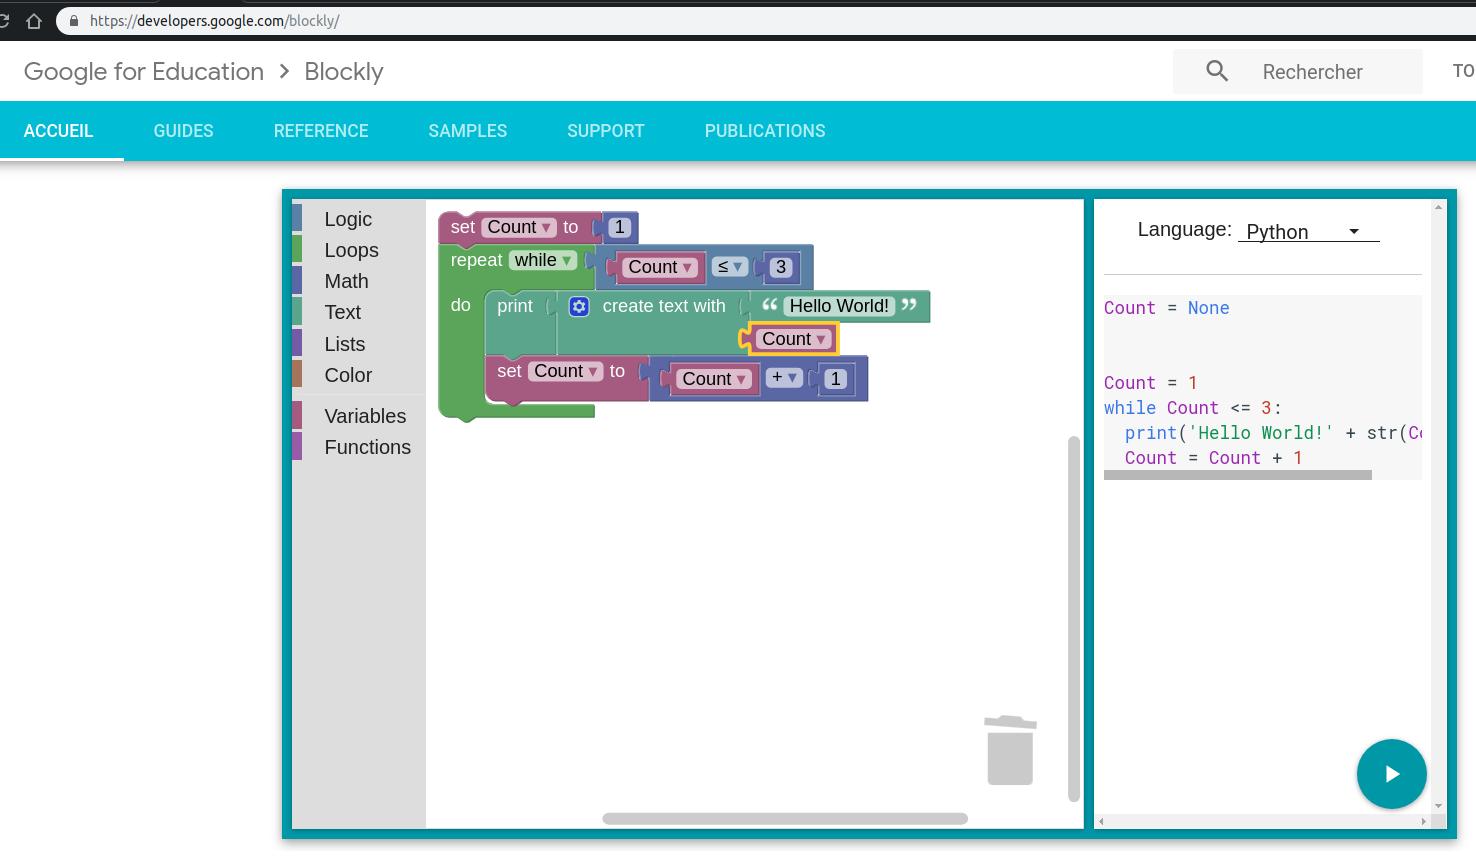
\includegraphics[height = .6\textheight]{blockly}
    \url{https://developers.google.com/blockly/}
  \end{center}
\end{frame}

\subsection{Python tutor}

\begin{frame}
  \begin{center}
    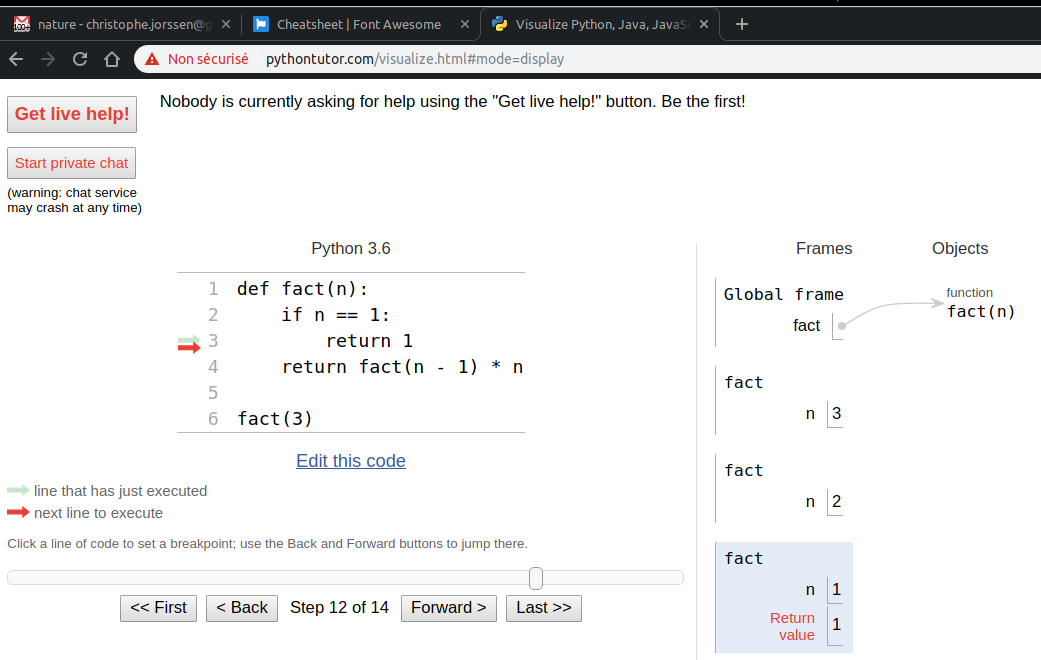
\includegraphics[height = .7\textheight]{python-tutor-fact}
    \url{http://pythontutor.com/visualize.html\#mode=edit}
  \end{center}  
\end{frame}

\miniframesoff

\section{}

\begin{frame}{Bibliographie}
  \begin{itemize}
  \item \emph{Informatique pour tous en CPGE}, Benjamin Wack \emph{et al.}, Eyrolles, 2013
  \item \emph{Data Structures and Algorithms in Python}, Michael T. Goodrich \emph{et al.}, Wiley, 2013
  \item \emph{Python Algorithms: Mastering Basic Algorithms in the Python Language}, Magnus Lie Hetland, APress, 2014
  \item PEP-8, \url{https://www.python.org/dev/peps/pep-0008/}
  \item \url{https://docs.scipy.org/doc/numpy/user/quickstart.html\#the-basics}
  \end{itemize}
\end{frame}

\end{document}

% Local Variables:
% coding: utf-8-unix
% TeX-engine: luatex
% End:
